\documentclass[]{book}
\usepackage{lmodern}
\usepackage{amssymb,amsmath}
\usepackage{ifxetex,ifluatex}
\usepackage{fixltx2e} % provides \textsubscript
\ifnum 0\ifxetex 1\fi\ifluatex 1\fi=0 % if pdftex
  \usepackage[T1]{fontenc}
  \usepackage[utf8]{inputenc}
\else % if luatex or xelatex
  \ifxetex
    \usepackage{mathspec}
  \else
    \usepackage{fontspec}
  \fi
  \defaultfontfeatures{Ligatures=TeX,Scale=MatchLowercase}
\fi
% use upquote if available, for straight quotes in verbatim environments
\IfFileExists{upquote.sty}{\usepackage{upquote}}{}
% use microtype if available
\IfFileExists{microtype.sty}{%
\usepackage{microtype}
\UseMicrotypeSet[protrusion]{basicmath} % disable protrusion for tt fonts
}{}
\usepackage[margin=1in]{geometry}
\usepackage{hyperref}
\hypersetup{unicode=true,
            pdftitle={Examining youth engagement during learning activities that involve work with data: An Experience Sampling approach},
            pdfauthor={Joshua M. Rosenberg},
            pdfborder={0 0 0},
            breaklinks=true}
\urlstyle{same}  % don't use monospace font for urls
\usepackage{natbib}
\bibliographystyle{apalike}
\usepackage{longtable,booktabs}
\usepackage{graphicx,grffile}
\makeatletter
\def\maxwidth{\ifdim\Gin@nat@width>\linewidth\linewidth\else\Gin@nat@width\fi}
\def\maxheight{\ifdim\Gin@nat@height>\textheight\textheight\else\Gin@nat@height\fi}
\makeatother
% Scale images if necessary, so that they will not overflow the page
% margins by default, and it is still possible to overwrite the defaults
% using explicit options in \includegraphics[width, height, ...]{}
\setkeys{Gin}{width=\maxwidth,height=\maxheight,keepaspectratio}
\IfFileExists{parskip.sty}{%
\usepackage{parskip}
}{% else
\setlength{\parindent}{0pt}
\setlength{\parskip}{6pt plus 2pt minus 1pt}
}
\setlength{\emergencystretch}{3em}  % prevent overfull lines
\providecommand{\tightlist}{%
  \setlength{\itemsep}{0pt}\setlength{\parskip}{0pt}}
\setcounter{secnumdepth}{5}
% Redefines (sub)paragraphs to behave more like sections
\ifx\paragraph\undefined\else
\let\oldparagraph\paragraph
\renewcommand{\paragraph}[1]{\oldparagraph{#1}\mbox{}}
\fi
\ifx\subparagraph\undefined\else
\let\oldsubparagraph\subparagraph
\renewcommand{\subparagraph}[1]{\oldsubparagraph{#1}\mbox{}}
\fi

%%% Use protect on footnotes to avoid problems with footnotes in titles
\let\rmarkdownfootnote\footnote%
\def\footnote{\protect\rmarkdownfootnote}

%%% Change title format to be more compact
\usepackage{titling}

% Create subtitle command for use in maketitle
\newcommand{\subtitle}[1]{
  \posttitle{
    \begin{center}\large#1\end{center}
    }
}

\setlength{\droptitle}{-2em}
  \title{Examining youth engagement during learning activities that involve work
with data: An Experience Sampling approach}
  \pretitle{\vspace{\droptitle}\centering\huge}
  \posttitle{\par}
  \author{Joshua M. Rosenberg}
  \preauthor{\centering\large\emph}
  \postauthor{\par}
  \predate{\centering\large\emph}
  \postdate{\par}
  \date{2018-06-12}

\usepackage{booktabs}
\usepackage{longtable}

\usepackage{amsthm}
\newtheorem{theorem}{Theorem}[chapter]
\newtheorem{lemma}{Lemma}[chapter]
\theoremstyle{definition}
\newtheorem{definition}{Definition}[chapter]
\newtheorem{corollary}{Corollary}[chapter]
\newtheorem{proposition}{Proposition}[chapter]
\theoremstyle{definition}
\newtheorem{example}{Example}[chapter]
\theoremstyle{definition}
\newtheorem{exercise}{Exercise}[chapter]
\theoremstyle{remark}
\newtheorem*{remark}{Remark}
\newtheorem*{solution}{Solution}
\begin{document}
\maketitle

{
\setcounter{tocdepth}{1}
\tableofcontents
}
\chapter{Introduction}\label{intro-placemarker}

Socializing, working, and even teaching and learning are increasingly
impacted by data. These sources of data--either quantitative \emph{or}
qualitative--are created by us, for us, and about us. Despite the
impacts of data, present opportunities for learners themselves to work
with data in educational settings are limited.

Work with data includes broad processes of collecting, creating,
modeling data, and even asking questions that can be answered with data.
This work, then, is more than just crunching numbers. It is also more
than interpreting a figure created by someone else. Rather, work with
data is about making sense of phenomena in the world--or solving
problems in the world. This focus on phenomena is particularly relevant
to those designing and enacting learning opportunities focused on work
with data (Lee \& Wilkerson, in press; Singer, Hilton, \& Schweingruber,
2006; Wild \& Pfannkuch, 1999).

Despite not being very widespread, aspects of work with data cut across
STEM (Science Technology Engineering and Mathematics) domains: Aspects
of work with data are recognized as core competencies across recent
curricular documents. They are found, for example, in the \emph{Next
Generation Science Standards} (NGSS Lead States, 2013) and the
\emph{Common Core State Standards} (in mathematics; National Governors
Association Center for Best Practices, Council of Chief State School
Officers, 2010). Both of these standards highlight the role of authentic
work with data.

Past research on work with data has largely been set in mathematics
contexts and has focused on mathematical practices, like generating
measures of phenomena and creating data models (English, 2012; Lehrer \&
Romberg, 1996; Lesh, Middleton, Caylor, \& Gupta, 2008). There has been
some research about work with data in science settings (Lee \&
Wilkerson, in press; National Research Council, 2012), though this work
varies greatly concerning the nature of work with data (McNeill \&
Berland, 2017). Findings from this past research broadly suggest that
engaging in work with data is powerful in terms of learning both about
and how to do mathematics and science. Lehrer and Schauble (2015),
summarizing past research on the use of mathematical practices in
science contexts, note that work with data ``has an exceptionally high
payoff in terms of students' scientific reasoning'' (Lehrer \& Schauble,
2015, p.~696).

To date, past research shows that using a framework from contemporary
engagement theory to characterize students' experiences has been
informative both in research and to practicing educators. Knowing more
about how youth engage in work with data is valuable as engagement is a
meaningful outcome for STEM learners in its own right (Sinatra, Heddy,
\& Lombardi, 2015). It may also be an antecedent of changes in other
outcomes, such as their well-being, achievement, and pursuit of an area
of study or career (Wang, Chow, Hofkens, \& Salmela-Aro, 2015; Wang \&
Eccles, 2012). However, research has not examined engagement in work
with data. Because engaging in work with data seems to be so potentially
beneficial to learners, better understanding the nature of work with
data and learners' engagement in such practices is needed.

The purpose of this study, then, is to examine youth engagement in a
variety of learning activities that involve work with data. Engagement
is explored in the context of outside-of-school STEM enrichment programs
carried out during the summer and work with data is considered through
the lens of specific aspects identified from past research, such as
asking questions and generating and modeling data. Knowing more about
how youth engage can also provide a foundation for subsequent work to
explore how particular curricula and engaging experiences for youth
spark their interest in work with data, including hobbies and
occupations related to data science, but also in STEM domains in
general.

\chapter{Literature Review}\label{literature-review}

The framework for this study is informed by work on STEM-related
learning practices, student engagement, and approaches to analyzing
complex psychological constructs, like engagement. In this review of the
literature, I define work with data as a key practice, or
learning-related activity, across STEM domains. I also define and
justify a multi-dimensional framework for understanding engagement, and
then review an approach to analyzing data that is ideal for capturing
this multidimensionality.

\section{Defining Work with Data}\label{defining-work-with-data}

Some scholars have focused on a few key pieces of data analysis,
connected through the use of ``data to solve real problems and to answer
authentic questions'' (Hancock et al., 1992, p.~337). This focus on
solving real problems or answering authentic questions--rather than
being taught and learned as isolated skills--is an essential part of
work with data having the most educational benefits to learners
(National Research Council, 2012; see Lehrer and Schauble {[}2012{]}
Windschitl, Thompson, \& Braaten {[}2018{]} for excellent, practice,
in-depth examples of work with data being used as part of instructional
approaches). This approach has primarily been used by mathematics
educators, as reflected in its role in statistics curriculum standards
(Franklin et al., 2007). In science settings, where answering questions
about phenomena serve as the focus of activities, it shares features of
the process of engaging in scientific and engineering practices but has
been less often studied.

Work with data has been conceived in different ways. For some specific
examples from different domains, see Lee and Wikerson's (in press)
forthcoming summary report for the National Academy of Sciences and Wild
and Pfannkuch (1999), Franklin et al. (2007), and Lehrer and Schauble
(2004). Because there is not an agreed-upon definition of work with
data--particularly across subject area domains (i.e., across all of the
STEM content areas)--I focus on the core aspects that scholars have most
often included in their conceptualizations of work with data. These core
components, synthesized from definitions across studies, are better for
understanding work with data across STEM content areas--as in the
present study--than the components from specific examples, which were
developed for use in only one domain. The aspects of work with data that
have been articulated in prior studies are distilled into five key
aspects (Figure 2.1) for use in this study. They are:

\begin{itemize}
\tightlist
\item
  \emph{Asking questions}: Generating questions that can be answered
  with empirical evidence
\item
  \emph{Making observations}: Watching phenomena and noticing what is
  happening concerning the phenomena or problem being investigated
\item
  \emph{Generating data}: The process of figuring out how or why to
  inscribe an observation as data about phenomena, as well as generating
  tools for measuring or categorizing
\item
  \emph{Data modeling}: Activities involving the use of simple
  statistics, such as the mean and standard deviation, as well as more
  complicated models, such as linear models and extensions of the linear
  model
\item
  \emph{Interpreting and communicating findings}: Activities related to
  identifying a driving question regarding the phenomena that the
  question is about
\end{itemize}

\begin{figure}

{\centering 
\includegraphics[width=0.8\linewidth]{images/figure1} 

}

\caption{Work with data in STEM education settings}\label{fig:unnamed-chunk-1}
\end{figure}

These five synthesized aspects of work with data are not stand-alone
practices but are a part of a cycle. This is not only because each
aspect follows that before it, but also because the overall process is
iterative: For example, interpreting findings often leads to new
questions and subsequent engagement in work with data. Also, scholars
have pointed out some key features of how work with data is carried out
that impact their effectiveness as a pedagogical approach. These key
features include an emphasis on making sense of real-world phenomena and
iterative cycles of engaging in work with data and collaboration and
dialogue, through which ideas and findings are critiqued and subject to
critique, and revised over time (McNeill \& Berland, 2017; Lee \&
Wilkerson, in press).

\section{The role of working with data in STEM learning
environments}\label{the-role-of-working-with-data-in-stem-learning-environments}

Working with data can serve as an organizing set of practices for
engaging in inquiry in STEM learning settings (Lehrer \& Schauble,
2015). Data are both encountered and generated by learners, and so
opportunities for learners to work with data provide many opportunities
to leverage their curiosity because processes of inquiry can be grounded
in phenomena that learners themselves can see and manipulate or
phenomena that learners are interested in. Also important, becoming
proficient in work with data can provide learners with an in-demand
capability in society, owing to the number of occupations, from
education to entrepreneurship, that demand or involve taking action
based on data (Wilkerson \& Fenwick, 2017). Furthermore, becoming
proficient in work with data can be personally empowering because of the
parts of our lives--from paying energy bills to interpreting news
articles--that use data.

Recent educational reform efforts emphasize work with data (i.e., the
scientific and engineering practices in the NGSS and the standards for
mathematical practice in the Common Core State Standards). However, work
with data is uncommon in many classroom settings, even classrooms
emphasizing recent science education reform efforts; McNeill \& Berland,
2017; Miller, Manz, Russ, Stroupe, \& Berland, in press). As a result,
learning environments suited to engaging in work with data, but not
explicitly designed to support it, may be valuable to study because they
may serve as incubators of these rare and challenging learning
activities.

Outside-of-school programs, in particular, are a potentially valuable
setting to explore engagement in work with data, because of the combined
pedagogical and technical expertise of their staff and the open-ended
nature of the activities that are possible to carry out during them.
Staff or youth activity leaders for these programs includes educators
and scientists, engineers, and others with the technical experience.
Additionally, the programs were designed to involve learners in the
types of real-world practices experienced by experts in STEM
disciplines. Attendance in such programs is associated with many
benefits to learners (Green, Lee, Constance, \& Hynes, 2013; see Lauer,
Akiba, Wilkerson, Apthorp, Snow, \& Martin-Glenn, 2006, for a
comprehensive review). These programs are also a good context for
understanding work with data because little research has examined how
data are part of the experiences of youth during them.

\section{What We Know (And Do Not Know) About How Youth Work with
Data}\label{what-we-know-and-do-not-know-about-how-youth-work-with-data}

There is a good amount of past research on cognitive capabilities as
outcomes from working with data. Much of this (laboratory-based)
research has focused on how children develop the capability to
inductively reason from observations (Gelman \& Markman, 1987). Other
research has focused on the development of causal, or mechanistic,
reasoning, among young children (Gopnik et al., 2001; Gopnik \& Sobel,
2000), often from a Piagetian, individual-development focused tradition
(i.e., Piaget \& Inhelder, 1969). A key outcome of engaging in work with
data has to do with how learners account for variability (Lehrer, Kim,
\& Schauble, 2007; Petrosino, Lehrer, \& Schauble, 2003; Lesh,
Middleton, Caylor, \& Gupta, 2008; Lee, Angotti, \& Tarr, 2010),
arguably the main goal of engaging in work with data (Konold \&
Pollatsek, 2002). From this research, we know that learners can develop
the capacity to reason about variability (and covariability).

Past research has also shown that there are strategies that can support
work with data. These include the design of technological tools and the
development of curricula. From this research, we know about specific
strategies and learning progressions for learners to develop this
capability, such as the role of measurement in exposing learners in a
direct way to sources of variability (Petrosino et al., 2003) or the
place of relevant phenomena, such as manufacturing processes, such as
the size of metallic bolts, which can help learners to focus on
``tracking a process by looking at its output'' (Konold \& Pollatsek,
2002, p.~282).

Finally, past research has shown that different aspects of work with
data pose unique opportunities and challenges. Asking empirical
questions requires experience and ample time to ask a question that is
both able to be answered with data and which is sustaining and worth
investigating (Bielik, 2016; Hasson \& Yarden, 2012). Making
observations and generating data, such as of the height of the school's
flagpole, requires negotiation not only of what to measure, but how and
how many times to measure it (Lehrer, Kim, \& Schauble, 2007). Regarding
modeling, not only teaching students about models, such as that of the
mean, but also asking them to create them, are valuable and practical
(Lehrer \& Schauble, 2004; Lehrer, Kim, \& Jones, 2011), but also
time-intensive. Interpreting findings, especially in light of
variability through models, and communicating answers to questions,
means not only identifying error but understanding its sources, and can
be supported through exploring models that deliberately represent the
data poorly, but can be instructive for probing the benefits and
weaknesses of models (Lee \& Hollebrands, 2008; Lehrer, Kim, \&
Schauble, 2007).

Despite the valuable past research that has been carried out, how
learners and youth participate in different aspects of work with data
through the lens of engagement theory has not been examined. Consider
the practice of modeling data, commonly described as a----or
\emph{the}----key part of many data analyses (Konold, Finzer, \&
Kreetong, 2017). When modeling data, learners may use data they
generated and structured in a data set on their own or may model
already-processed, or use already-plotted, data (McNeill \& Berland,
2017). How challenging do students perceive the different enactments of
these activities to be and how do learners perceive their competence
regarding them? Importantly, how hard are learners working? How much do
they feel they are learning? Knowing more about these beliefs,
characteristics, and processes could help us to develop informed
recommendations for teachers and designers intending to bring about
opportunities for learners to engage in work with data in a
better-supported way that is sustained over time.

\section{Engagement in General and in STEM
Domains}\label{engagement-in-general-and-in-stem-domains}

In this section, the nature of engagement is discussed in terms of
general features that have been identified across content area domains,
conditions that support engagement, and differences between engagement
in general and in STEM settings. This is followed by a discussion of two
key features of engagement: its dynamic, or context-dependent,
characteristics, and its multidimensional nature. Finally, I describe
methods for capturing these two features \emph{empirically} through an
approach called the Experience Sampling Method, or ESM, and describe how
multidimensional data, collected by ESM, can be analyzed.

Engagement is defined in this study as active involvement, or
investment, in activities (Blumenfeld et al., 2004). Explaining how
learners are involved in activities and tasks is especially important if
we want to know about what aspects of work with data are most engaging
(and in what ways), and therefore can serve as examples for others
advancing work with data as well as those calling for greater support
for engagement. Apart from being focused on involvement, engagement is
often thought of as a meta-construct, that is, one that is made up of
other constructs (Skinner \& Pitzer, 2012; Skinner, Kindermann, \&
Furrer, 2009). By defining engagement as a meta-construct, scholars
characterize it in terms of cognitive, behavioral, and affective
dimensions that are distinct yet interrelated (Fredricks, 2016).

We know from past research that the cognitive, behavioral, and affective
dimensions of engagement can be distinguished (Wang \& Eccles, 2012;
Wang \& Holcombe, 2012) and that while there are long-standing concerns
about the conceptual breadth of engagement (Fredricks et al., 2016),
careful justification and thoughtful use of multidimensional engagement
constructs and measures is warranted. Engagement is also considered to
be changing in response to individual, situation or moment contextual
factors, Skinner and Pitzer's (2012) model of motivational dynamics,
highlighting the community, school, classroom, and even learning
activity, shows the context-dependent nature of engagement on the basis
of the impacts of these factors on learners' engagement.

Engagement in STEM settings shares characteristics with engagement
across disciplines, yet there are some distinct aspects to it (Greene,
2015). While one type of engagement---behavioral---is associated with
achievement-related outcomes, many STEM practices call for engagement in
service of other outcomes, especially around epistemic and
agency-related dimensions (Sinatra et al., 2015,). For example, many
scholars have defined scientific and engineering practices as cognitive
practices, which involve applying \emph{epistemic considerations} around
sources of evidence and the nature of explanatory processes (see Berland
et al. 2016, Stroupe, 2014; Miller et al., in press).

The emphasis on developing new knowledge and capabilities by engaging in
STEM practices must be reflected in how the cognitive dimension of
engagement is measured. Because of the importance of constructing
knowledge to engagement in STEM practices, then, cognitive engagement is
defined for this study in terms of learning something new or getting
better at something. While sometimes defined in terms of
extra-curricular involvement or following directions, behavioral
engagement is defined in this study as working hard on learning-related
activities (Fredricks et al., 2004; Singh, Granville, \& Dika, 2002).
Finally, affective engagement is defined as affective responses to
activities, such as being excited, angry, or relaxed (Pekrun \&
Linnenbrink-Garcia, 2012).

Finally, some key conditions that facilitate engagement. Emergent
Motivation Theory (EMT; Csikszentmihalyi, 1990), provides a useful lens
for understanding these conditions. From EMT, a key condition for
engagement that can change dynamically, from moment to moment, is how
difficult individuals perceive an activity to be, or its \emph{perceived
challenge}. Another key condition is how good at an activity individuals
perceive themselves to be, or their \emph{perceived competence}. What is
most important--and necessary in terms of being engaged--is being both
challenged by and good at a particular activity.

Past research has supported this conjecture (Csikszentmihalyi, 1990). As
one empirical example, Shernoff et al. (2016) demonstrated that the
interaction of challenge and competence was associated with positive
forms of engagement. These findings suggest that learners' perceptions
of the challenge of the activity, and their perceptions of how skillful
they are, are important conditions that co-occur with learners'
engagement. Conceptualizing perceptions of challenge and competence as
conditions, rather than factors that influence engagement, is in
recognition of their co-occurrence within individuals, in that youth
experience engagement and their perceptions of the activity (perceived
challenge) and of themselves (perceive competence) together and at the
same time. Thus, these two conditions (challenge and competence) are
considered together with engagement in this study, as described in the
section below on analyzing multidimensional data on engagement.

\section{Youth characteristics that may affect their
engagement}\label{youth-characteristics-that-may-affect-their-engagement}

Past research suggests learners or youths' characteristics, such as
their interest in the domain of study, impact their cognitive,
behavioral, and affective engagement (Shernoff et al., 2003; Shernoff et
al., 2016; Shumow, Schmidt, \& Zaleski, 2013). These are both
moment-to-moment, context-dependent conditions that support engagement
(like those discussed above, perceptions of challenge and competence) as
well as youth-specific factors. These factors are at the level of
individual differences (i.e., youths' more stable interest in STEM
domains), and may impact engagement, as described in this section.

A factor that can support engagement is how teachers support learning
practices (Strati, Schmidt, \& Maier, 2017). Particularly concerning
work with data, which is demanding not only for learners but also
teachers (Lehrer \& Schauble, 2015; Wilkerson, Andrews, Shaban, Laina,
\& Gravel, 2016), sustained support from those leading youth activities
is an essential component of learners being able to work with data.
Thus, how youth activity leaders plan and enact activities related to
work with data can have a large impact on students' engagement.
Furthermore, because of the importance of work with data across STEM
domains, carrying out ambitious activities focused on work with data may
plausibly have a substantial impact on the extent to which youth engage
in summer STEM program settings. Consequently, this study considers work
with data through the use of a coding frame that characterizes the
extent to which teachers are supporting specific STEM practices in their
instruction, including aspects of work with data.

Other factors that impact youths' engagement are individual
characteristics and differences. In recognition of differences among
learners in their tendency to engage in different (higher or lower) ways
in specific activities based in part on individual differences (Hidi \&
Renninger, 2006), learners' interest in STEM before the start of the
programs is also considered as a factor that can impact engagement.
Knowing about whether and to what extent youths' interest \emph{before}
participating in summer STEM programs explains their engagement
\emph{during} them is a key question in its own right. It is also
important in terms of properly understanding the effects of other
factors, such as working with data, above and beyond the effect of
pre-program interest. In addition to this interest, gender and the
racial and ethnic group of students is also considered, as past research
has indicated these as factors that influence engagement in STEM
(Bystydzienski, Eisenhart, \& Bruning, 2015; Shernoff \& Schmidt, 2008).
To include the racial and ethnic group of students, being part of an
under-represented minority (URM) group is considered. To sum up, youths'
pre-program interest, gender, and URM group membership are considered as
individual factors that may impact youths' engagement.

\section{Challenges of Measuring Engagement as a Contextually-Dependent
and Multidimensional
Construct}\label{challenges-of-measuring-engagement-as-a-contextually-dependent-and-multidimensional-construct}

Because of the way engagement has been thought of as having
context-dependent characteristics and being multi-dimensional, it is
challenging to use engagement (when conceptualized in such a way) in
empirical studies. One methodological approach that has benefits in
terms of both the context-dependent and multidimensional nature of
engagement is the ESM. Some scholars have explored or extolled benefits
to its use in their recent work (e.g., Strati et al., 2017; Turner \&
Meyer, 2000; Sinatra et al., 2015).

This study employs the Experience Sampling Method (ESM; Hektner,
Schmidt, \& Csikszentmihalyi, 2007) where learners answer short
questions about their experience when signaled. ESM involves asking
(usually using a digital tool and occasionally a diary) participants
short questions about their experiences. ESM is particularly well-suited
to understanding the context-dependent nature of engagement because
students answered brief surveys about their experience when they were
signaled, minimally interrupting them from the activity they are engaged
in and also seeking to collect measures about learners' experience when
signaled (Hektner et al., 2007).

The ESM approach is both sensitive to changes in engagement over time,
as well as between learners and allows us to understand engagement and
how factors impact it in more nuanced and complex ways (Turner \& Meyer,
2000). Though time-consuming to carry out, ESM can be a robust measure
that leverages the benefits of both observational and self-report
measures, allowing for some ecological validity and the use of
closed-form questionnaires amenable to quantitative analysis
(Csikszentmihalyi \& Larson, 1987). Despite the logistic challenge of
carrying out ESM in large studies, some scholars have referred to it as
the \emph{gold standard} for understanding individual's subjective
experience (Schwarz, Kahneman, \& Xu, 2009).

Research has shown us how the use of ESM can lead to distinct
contributions to our understanding of learning and engagement. This work
also suggests how ESM can be put to use for the present study. For
example, Shernoff, Csikszentmihalyi, Schneider, and Shernoff (2003)
examined engagement through the use of measures aligned with flow
theory, namely, using measures of concentration, interest, and enjoyment
(Csikszentmihalyi, 1997). In a study using the same measures of
engagement (Shernoff et al. (2016) used an observational measure of
challenge and control (or environmental complexity) and found that it
significantly predicted engagement, as well as self-esteem, intrinsic
motivation, and academic intensity. Schneider et al. (2016) and
Linnansaari et al. (2015) examined features of optimal learning moments
or moments in which students report high levels of interest, skill, and
challenge, as well as their antecedents and consequences. Similar to ESM
in that through its use engagement can be studied in a more
context-sensitive, still other scholars have used daily diary studies to
examine engagement as a function of autonomy-supportive classroom
practices (Patall, Vasquez, Steingut, Trimble, \& Pituch, 2015; Patall,
Steingut, Vasquez, Trimble, \& Freeman, 2017). This past research that
used ESM (or daily diary studies) to study engagement has shown that ESM
can be used to understand fine-grained differences in learning
activities, such as the aspects of work with data that are the focus of
this study.

Other research shows us that there are newer approaches to analyzing ESM
data that can contribute insights into the context-dependent nature of
engagement in a more fine-grained way. For example, Strati et al. (2017)
explored the relations between engagement to measures of teacher
support, finding associations between instrumental support and
engagement and powerfully demonstrating the capacity of ESM to
understand some of the context-dependent nature of engagement.
Similarly, Poysa et al. (2017) used a similar data analytic approach as
Strati et al. (2017), that is, use of crossed effects models for
variation within both students and time points, both within and between
days. These studies establish the value of the use of ESM to understand
the context-dependent nature of engagement and that such an approach may
be able to be used to understand engaging in work with data.
Additionally, these recent studies (particularly the study by Strati and
colleagues) show that how effects at different levels are treated,
namely, how variability at these levels is accounted for through random
effects as part of mixed effects models, is a key practical
consideration for the analysis of ESM data.

One powerful and increasingly widely used way to examine
context-dependent constructs, such as engagement, is the use of
\emph{profiles of}, or groups of variables that are measured. This
profile approach is especially important given the multidimensional
nature of engagement. In past research, profiles are commonly used as
part of what is described as person-oriented approaches (see Bergman \&
Magnusson, 1997), those used to consider the way in which psychological
constructs are experienced together and at once in the experiences of
learners. Note that in the present study, ESM involves asking youth
about to report on their experience at the time they were signaled
(rather than, for example, before or after the program, which
traditional surveys are well-suited for).

In this study, \emph{profiles of engagement} are used in the service of
understanding how students engage in work with data in a more holistic
way. There are some recent studies taking a profile approach to the
study of engagement (i.e., Salmela-Aro, Moeller, Schneider, Spicer, \&
Lavonen, 2016a; Salmela-Aro, Muotka, Alho, Hakkarainen, \& Lonka, 2016b;
Van Rooij, Jansen, \& van de Grift, 2017; Schmidt, Rosenberg, \& Beymer,
2018), though none have done so to study youths' engagement in work with
data.

The profile approach has an important implication for how we analyze
data collected from ESM about youths' engagement, in particular when we
consider how to understand engagement as a multi-dimensional construct,
and one with momentary, or instructional episode-specific, conditions
(Csikszentmihalyi, 1990). We know from past research that engagement can
be explained in terms of different patterns among its components
(Bergman \& Magnusson, 1997), in the present case its cognitive,
behavioral, and affective components. Because learners' engagement
includes cognitive, behavioral, and affective aspects experienced
together at the same time, it can be experienced as a combined effect
that is categorically distinct from the effects of the individual
dimensions of engagement. This combined effect can be considered as
profiles of engagement.

Past studies have considered profiles of cognitive, behavioral, and
affective aspects of engagement. For example, to account for the
context-dependent nature of engagement, some past studies have used
other measures to predict engagement, such as the use of in-the-moment
resources and demands (Salmela-Aro et al., 2016b) and the use of
instructional activities and choice (Schmidt et al., 2018). A potential
way to extend this past research is to account for not only engagement
(cognitive, behavioral, and affective), but also the intricately
connected perceptions of challenge and competence. This is especially
important since a profile approach emphasizes the holistic nature of
engagement and the impact of not only external but also intra-individual
factors. Accordingly, youths' perceptions of the challenge of the
activity and their competence at it are used along with the measures of
engagement to construct profiles of engagement. Thus, the profiles of
engagement include youths' responses to five ESM items for their
cognitive, behavioral, and affective engagement and their perceptions of
how challenging the activity they were doing is and of how competent at
the activity they are.

\section{Need for the Present Study}\label{need-for-the-present-study}

While many scholars have argued that work with data can be understood in
terms of the capabilities learners develop and the outcome learners
achieve, there is a need to understand learners' experiences working
with data. The present study does this through the use of contemporary
engagement theory and innovative methodological and analytic approaches.
Doing this can help us to understand work with data in terms of
learner's experience, which we know from past research impacts what and
how students learn (Sinatra et al., 2015). Knowing more about students'
engagement can help us to design activities and interventions focused
around work with data. In addition to this need to study engagement in
work with data through the lens of engagement, no research has yet
examined work with data in the context of summer STEM programs, though
such settings are potentially rich with opportunities for highly engaged
youth to analyze authentic data sources.

\section{Conceptual Framework and Research
Questions}\label{conceptual-framework-and-research-questions}

To sum up, the present study is about how learning activities involving
various aspects of work with data can be understood in terms of
engagement. Its context is out-of-school-time STEM enrichment programs
designed to meet guidelines for best practices. The conceptual framework
in the present study is presented in Figure 2.2 and is laid out in the
remainder of this section.

There are five aspects of work with data synthesized from past research
(i.e., Hancock et al., 1992; Lehrer \& Romberg, 1996; Wild \& Pfannkuch,
1999):

\begin{enumerate}
\def\labelenumi{\arabic{enumi}.}
\tightlist
\item
  Asking questions or identifying problems
\item
  Making observations
\item
  Generating data
\item
  Data modeling
\item
  Interpreting and communicating findings
\end{enumerate}

In Figure 2.2, engagement in work with data is associated with different
profiles of engagement. The theoretical framework for the profile
approach suggests that engagement is a multi-dimensional construct
consisting of cognitive, behavioral, and affective dimensions of
engagement and perceptions of challenge and competence. Also, a
pre-program measure of youths' pre-program interest in STEM, along with
youths' gender and URM status, are hypothesized to be associated with
the profiles and the relations of work with data and the profiles.

\begin{figure}

{\centering 
\includegraphics[width=0.8\linewidth]{images/figure2} 

}

\caption{A conceptual framework for this study and research questions}\label{fig:unnamed-chunk-2}
\end{figure}

Regarding research questions 2-5, the ESM responses that make up the
profiles are associated with different ``levels.'' These \emph{levels},
or groups, which may introduce dependencies that violate statistical
assumptions of the independence of the responses, are commonly
considered in the Hierarchical Linear Modeling (also known as
multi-level or mixed effects modeling) literature as \emph{random
effects} (Gelman \& Hill, 2007; West, Welch, \& Galecki, 2015). In this
study, three levels that can be modeled as random effects to account for
the dependencies they introduce: Youth, instructional episode (which are
indicators for the moments--or segments--in which youth are asked to
respond to the ESM signal), and the program. Thus, these are not
predictor variables, but rather are the levels that are present given
the approach to data collection and the sampling procedure. Interpreting
their effects is not a goal of this study, but accounting for them in
the models used, as in this study, is essential and and is done through
the use of random effects.

Pre-program interest, gender, and URM status are predictor variables at
the youth level. The aspects of work with data are predictor variables
at the instructional episode level. There are no predictor variables at
the program level, in part due to the small number of programs (and the
resulting low statistical power of any variables added at this level).
To summarize, pre-program interest, gender, and URM status, and the
aspects of work with data are used as predictor variables, while the
three levels (youth, instructional episode, and program) are accounted
for in the modeling strategy.

The five research questions, then, are:

\begin{enumerate}
\def\labelenumi{\arabic{enumi}.}
\tightlist
\item
  What is the frequency and nature of opportunities for youth to engage
  in each of the five aspects of work with data in summer STEM programs?
\item
  What are sources of variability for the profiles of engagement?
\item
  What profiles of engagement emerge from data collected via ESM in the
  programs?
\item
  How do the five aspects of work with data relate to profiles of
  engagement?
\item
  How do youth characteristics relate to profiles of engagement?
\end{enumerate}

\chapter{Method}\label{method}

\section{Context}\label{context}

The setting for the present study was nine out-of-school STEM programs
during 2015 in the Northeast United States. Two \emph{intermediary
organizations} which were contracted by the local school districts to
administer the summer programs. The two intermediaries were responsible
for soliciting and enrolling youth; establishing guidelines for the
design of the programs, and the goals of the programs; and providing
training and professional development for the staff, hereafter referred
to as youth activity leaders.

There was a difference between the two intermediary organizations,
namely, one \emph{separated academic and enrichment-related activities},
whereas, in the other, the \emph{academic and enrichment components were
more integrated}, which may have program-related effects on youths'
engagement. Many of the programs aim to involve youth in work with data.
These learning environments bring together youth activity leaders,
educators, and those with technical expertise in STEM domains. Youth
spent around three hours per day for four days per week for the
approximately four-week programs, which were taught by youth activity
leaders and scientists, engineers, and other community members with
technical expertise.

\section{Participants}\label{participants}

Participants consisted of 203 youth. Participants were from diverse
racial and ethnic backgrounds (see Table 3.1). The mean age of
participants was around 13 years old (from youth whose age was
available: \emph{M} = 12.71, \emph{SD} = 1.70, \emph{min.} = 10.75,
\emph{max.} = 16.36). Detailed demographic characteristics of youth are
presented in Table 3.1.

\begin{table}

\caption{\label{tab:unnamed-chunk-3}Demographic characteristics of youth}
\centering
\begin{tabular}[t]{lr}
\toprule
Youth & Percentage\\
\midrule
Sex & \\
Male & 50\\
Female & 50\\
Race/Ethnicity & \\
Hispanic & 48\\
\addlinespace
White & 6\\
Black & 36\\
Multi-racial & 3\\
Asian/Pacific Islander & 7\\
Parent Education & \\
\addlinespace
High School or Below & 79\\
Graduated from College (B.A. or B.S.) & 21\\
\bottomrule
\end{tabular}
\end{table}

\section{Procedure}\label{procedure}

Before the start of the programs, youth completed a pre-survey that
included questions about their experience in STEM, intention to pursue a
STEM major or career, and other motivation and engagement-related
measures.

At the beginning of the programs, youth were introduced to the study and
the phones used for data collection related to the ESM. As indicated in
the earlier section, ESM is a method of data collection that involves
asking youth to respond to short questions on phones (that were provided
as part of the study). In particular, youth were signaled at random
times (within intervals, so that the signals were not too near or far
apart) in order to obtain a sample of their experience throughout the
program. ESM data were collected two days each week, for three weeks
(weeks 2-4 of the program). In all of the programs, about equal
video-recording time was dedicated to classroom and field experiences.
This detail is noteworthy because programs associated with one of the
intermediaries rotated between classroom and field experience days,
while the other used the first half of each day for one and the second
for the other. Each day, youth were signaled four times. These signals
were at the same time for all of the youth within their program, but at
different times between programs and between days within programs (with
the constraint that no two signals could occur less than ten minutes
apart).

The programs were video-recorded by research team members on the days
during which ESM data were collected. So that the measures relating the
video-recording and ESM data can be matched, the videos included a
signal from the video-recorder that identified the ESM signal to which
youth responded.

\section{Data Sources and Measures}\label{data-sources-and-measures}

Data sources consist of ESM measures of engagement and youths'
perceptions of themselves and the activity, pre-survey measures of
youths' interest, youths' demographic information, and the
video-recordings of programs.

\subsection{ESM measures of engagement for the
profiles}\label{esm-measures-of-engagement-for-the-profiles}

Measures for engagement were created from five ESM questions, three
serving indicators for the experience of engagement and two for the
conditions of engagement. The three indicators for engagement were for
learning (for the cognitive engagement construct), working hard (for
behavioral engagement), and enjoying (for affective engagement). The
variables for the conditions are for perceived challenge and perceived
competence.

All five items are ultimately used to construct the profiles of engaged.
Each of the ESM items consisted of the item text and the following four
item response options, of which youth were directed to select one: Not
at all (associated with the number 1 on the survey; 1), A little (2),
Somewhat (3), and Very Much (4), as presented in Table 3.2. Note that
because these items are measured using single-item indicators (which is
common in studies using ESM; Hektner et al., 2007), information about
the reliability and validity information for these measures is not
included.

\begin{table}

\caption{\label{tab:unnamed-chunk-4}ESM measures for profiles}
\centering
\resizebox{\linewidth}{!}{\begin{tabular}[t]{ll}
\toprule
Construct & Item\\
\midrule
Cognitive engagement & As you were signaled, were you learning anything or getting better at something?\\
Behavioral engagement & As you were signaled, how hard were you working?\\
Affective engagement & As you were signaled, did you enjoy what you are doing?\\
Perceived challenge & As you were signaled, how challenging was the main activity?\\
Perceived competence & As you were signaled, were you good at the main activity?\\
\bottomrule
\end{tabular}}
\end{table}

\subsection{The five aspects of work with
data}\label{the-five-aspects-of-work-with-data}

Different aspects of work with data are identified from
video-recordings. Specifically, codes for work with data were generated
on the basis of the activity that the youth activity leaders were
facilitating. The activity youth activity leaders were facilitating were
from the STEM-Program Quality Assessment (STEM-PQA; Forum for Youth
Investment, 2012), an assessment of quality programming in after-school
programs. I then identified the specific activities that corresponded to
the five aspects of work with data, as defined in Table 3.4. Details on
the reliability of this measure are described next; more information on
how the measure aligns with the original STEM-PQA on which this measure
is based are presented in Appendix A.

Raters contracted by American Institute of Research (AIR) were trained
in the use of the Program Quality Assessment tool (PQA)--the broader
assessment tool for which the STEM-PQA is a supplement. Raters completed
a four-hour online training module on the overall PQA tool and then
attended an in-person two-day training led by a trainer from the David
P. Weikart Center for Youth Program Quality, the tool's publisher, where
they learned about the instrument, trained on its use, and then
established inter-rater reliability with a master coder. For the
STEM-PQA, three of the same raters contracted by AIR to code the
(overall) PQA measure used the STEM-PQA supplement to score one video
segment, for which there were no disagreements on scoring for any of the
items. The programs were divided up among all of the raters, so raters
coded some of the videos for all of the programs. When the raters
encountered a situation that was difficult to score, they would all
discuss the issue by telephone or more often by email after viewing the
video in question and reach a consensus on how to score the specific
item. Note that these codes were unique to each signal to which youth
responded (but were not unique to each youth, as youth in the same
program were signaled at the same time).

Out of the 248 instructional episodes, 236 were code-able for work with
data; for the 12 that were not codeable, issues with the
video-recordings were the primary source of the missing data. These 236
responses are used for all of the analyses.

\begin{landscape}\begin{table}

\caption{\label{tab:unnamed-chunk-5}Coding Frame for Work With Data}
\centering
\resizebox{\linewidth}{!}{\begin{tabular}[t]{ll}
\toprule
Code & Description\\
\midrule
Asking questions & Discussing and exploring topics to investigate and pose questions.\\
Making observations & Watching and noticing what is happening with respect to the phenomena or problem being investigated.\\
Generating data & Figuring out how or why to inscribe an observation as data and generating coding frames or measurement tools.\\
 & \\
Data modeling & Understanding and explaining phenomena using models of the data that account for variability or uncertainty.\\
Interpreting and communicating findings & Discussing and sharing and presenting findings.\\
\bottomrule
\end{tabular}}
\end{table}
\end{landscape}

\subsection{Survey measures of pre-interest in
STEM}\label{survey-measures-of-pre-interest-in-stem}

Measures of youths' pre-interest are used as youth-level characteristics
that predict the profiles of engagement. In particular, three items
adapted from Vandell, Hall, O'Cadiz, and Karsh (2012) were used, with
directions for youth to rate their agreement with the items' text using
the same scale as the ESM items: Not at all (associated with the number
1 on the survey), A little (2), Somewhat (3), and Very Much (4).
Reliability and validity information on this scale is presented in
Vandell et al. (2008).

This measure was constructed by taking the maximum value for the scales
for the different content areas (science, mathematics, and engineering),
so that the value for a youth whose response for the science scale was
2.5 and for the mathematics scale was 2.75 would be 2.75. See Beymer,
Rosenberg, and Schmidt (2018) for more details on this (taking the
maximum value) measurement approach. The items are presented in Table
3.3. Overall levels of this measure were high (\emph{M} = 3.044
(\emph{SD} = 0.901).

\begin{table}

\caption{\label{tab:unnamed-chunk-6}Measure for pre-program interest in STEM}
\centering
\begin{tabular}[t]{ll}
\toprule
Construct & Items.text\\
\midrule
Pre-program interest in STEM & I am interested in science / mathematics / engineering.\\
 & At school, science / mathematics / engineering is fun\\
 & I have always been fascinated by science / mathematics / engineering)\\
\bottomrule
\end{tabular}
\end{table}

\subsection{Other youth
characteristics}\label{other-youth-characteristics}

In addition to the measures described in this section, demographic
information for youths' gender and their racial and ethnic group are
used to construct demographic variables for gender and membership in an
under-represented (in STEM) group; membership in an under-represented
group is identified on the basis of youths' racial and ethnic group
being Hispanic, African American, Asian or Pacific Islanders, or native
American.

\section{Data Analysis}\label{data-analysis}

\subsection{Preliminary analyses}\label{preliminary-analyses}

Correlations (first-order Pearson) and the frequency, range, mean
(\emph{M}), and standard deviation (\emph{SD}) are first presented for
all variables. In addition, the frequency of the codes for aspects of
work with data and the numbers of responses by youth, program, and
instructional episode are presented.

\subsection{Analysis for Research Question \#1 (on the frequency and
nature of work with
data)}\label{analysis-for-research-question-1-on-the-frequency-and-nature-of-work-with-data}

There were two primary steps taken to answer this question, one more
quantitative in nature and one more qualitative. The quantitative aspect
focused on the frequency of work with data, whereas the qualitative
aspect focused on the specific nature of work with data.

For the quantitative aspect, the codes for the aspects of work with data
(described above in the section on the measures) were counted up and
presented as a proportion of the number of code-able instructional
episodes. As the signals represent a sample of youths' experiences in
the programs, results from this analysis provide insight into how often
each of the aspects took place during the programs. Note that this
coding frame focused on the degree of \emph{instructional support} the
activity leaders provided for youth to work with data, thus results from
this analysis will show how often support for the different aspects of
work with data was provided, though youth may engage in the aspects of
work with data to varying degrees.

The frequency of work with data, the focus of the quantitative analysis
for this research question, will provide insight into how regular the
aspects of work with data are, but not about the ways in which work with
data was enacted. For example, qualitative differences in \emph{how}
youth were asking questions will not be evident from the codes as they
are used. In order to provide more detail in terms of the nature of work
with data in summer STEM segments, the data was coded with an
open-ended, qualitative approach.

Specifically, three research assistants were trained for approximately
eight hours, over the course of four meetings. Then, each research
assistant coded all of the segments associated with the videos for a
particular. Two coders coded every segment, except for the segments for
which the quantitative coding indicated no aspects of work with data
were present; instead, for these segments, only one coder coded each
segment.

The coders used the following five guiding questions, associated with
each of the five aspects of work with data, for the qualitative coding:

\begin{itemize}
\tightlist
\item
  When questioning or defining problems was observed, what types of
  questions/problems were involved?
\item
  When making observations is coded, what is the focus of observing?
\item
  When generating data is coded, what is being collected or recorded?
\item
  When analyzing or modeling data is coded, what analysis is being done,
  or what models are used?
\item
  When interpreting and communicating findings is coded, what is being
  interpreted or communicated?
\end{itemize}

For all of the guiding questions, the coders also took note of
\emph{who} (the youth, youth activity leader, or someone else) was the
focus of the aspect of work with data. For example, with respect to
interpreting and communicating findings, denoted when youth were sharing
the results from a hands-on investigation or when it was the youth
activity leader doing so as a summary on the basis of the work youth
recently completed.

After coding all of the segments for each program, the coders and I met
to discuss potential issues that emerged throughout the coding. The goal
of the meetings was to address any problems encountered when using the
guiding questions and to clarify how they applied the coding frame.
After the coding was complete, I then read through all of the codes for
all of the segments then made notes associated with each of the five
aspects of work with data. I used these notes to write descriptions of
the nature of work with data for each of the five aspects. After reading
through the qualitative codes and my descriptions of the nature of work
with data during each segment, I grouped the descriptions into themes,
which I present in the results for this research question. I also used
these themes to calculate proportions, which are also presented in the
findings for this section. In summary, an open-ended, qualitative coding
approach was used to create descriptions of the ways in which each of
the aspects of work with data was enacted. This analysis is used to
provide insights into the nature of work with data in summer STEM
programs.

\subsection{Analysis for Research Question \#2 (what profiles of
engagement
emerge)}\label{analysis-for-research-question-2-what-profiles-of-engagement-emerge}

Latent Profile Analysis (LPA; Harring \& Hodis, 2016; Muthen, 2004) is
used to identify profiles of engagement. LPA allows for capturing the
multidimensional nature of engagement through profiles in terms of
discovering groups of the ways in which youth experience engagement
together and at once.. A key benefit of the use of LPA, in addition to
likelihood estimation-based fit indices, is probabilities of an
observation being a member of a cluster (unlike in cluster analysis).
These profiles make it possible to analyze the multivariate data
collected on engagement in a way that balances the parsimony of a single
model.

For these analyses, five variables were included: the three indicators
for the experience of engagement (cognitive, behavioral, and affective)
and the two necessary conditions for it (perceptions of challenge and
competence). In addition, solutions with between two and 10 profiles
were considered. As part of LPA, the model type selection--where the
type refers to which parameters are estimated--is a key topic. For the
present study, six model types were considered:

\begin{enumerate}
\def\labelenumi{\arabic{enumi}.}
\tightlist
\item
  Varying means, equal variances, and covariances fixed to 0
\item
  Varying means, equal variances, and equal covariances
\item
  Varying means, varying variances, and covariances fixed to 0
\item
  Varying means, varying variances, and equal covariances
\item
  Varying means, equal variances, and varying covariances
\item
  Varying means, varying variances, and varying covariances
\end{enumerate}

The MPlus software (Muthen \& Muthen, 1998-2017) is used to carry out
LPA through statistical software I developed, \emph{tidyLPA}. More
details on LPA are included in Appendix D.

To select a solution in terms of the model type and the number of
profiles to be interpreted and used in subsequent analyses, a number of
fit statistics and other considerations were taken into account. These
include a range of information criteria (AIC, BIC, sample adjusted BIC
{[}SABIC{]}, consistent AIC {[}CAIC{]}), statistics about the quality of
the profile assignments (entropy, which represents the mean posterior
probability), statistical tests (Vu-Lo-Mendell-Rubin LRT {[}VLMR{]},
Lo-Mendell-Rubin LRT {[}LMR{]}, and the bootstrapped LRT {[}BLRT{]}),
and concerns of interpretability and parsimony are used. On the basis of
these criteria, a particular solution is selected and used as part of
subsequent analyses; as the model selection process is an integral part
of providing an answer to this question, the model and number of
profiles selected are described in the section for the results for this
research question.

\subsection{Analysis for Research Question \#3 (sources of variability
for the
profiles)}\label{analysis-for-research-question-3-sources-of-variability-for-the-profiles}

How youth are engaging is a function of who they are as an individual,
what they happen to be doing during a particular instructional episode,
and which youth program they are enrolled in, as well as random
variation. This analysis seeks to identify how much of the variation is
at each of these levels through using null models, or models only with
the indicators for the three levels (youth, instructional episode, and
program). These models can show how much variability in the profiles is
systematic at these different levels and is potentially attributable to
each of these types of factors. These null models may also suggest
something about where you might want to be looking to explain sources of
youth's engagement.

Sources of variability in these profiles can be used as additional
information in their own right for interpreting the profiles and in
order to anticipate the effects of predictor variables at the youth,
instructional episode, and program levels. First, the proportion of the
variability at each of these levels is explored through the use of null,
or variance components, in Table 4.4. These are models that only include
grouping (i.e., the variable identifying which youth a response is from,
what signal the response is associated with, and from which program the
youth and signal were from) factors. These models provide insight into
at which of these ``levels'' predictors may be able to explain the
outcome.

Variability in terms of the number (and proportion) of profiles each
youth reports can also be considered. The breakdown of responses in each
of the six profiles by youth is used to show the extent to which youth
report their most reported profile. In addition, apart from this overall
mean proportion of youths' responses, the mean proportion for specific
profiles (i.e., when youth report a particular profile the most, how
often, on average, do they report it?) are also considered.

The \emph{ICC}s provide information about sources of variability in the
profiles of engagement with respect to the same profile. One way to
better understand the nature of variability across profiles is by
examining how often youth reported the same profile: Whether youth
exhibit stable or highly variables modes of engagement (i.e., are some
youth always \emph{Fully} engaged?) can provide a descriptive portrait
of youths' experiences the many instructional episodes they were
involved in. To determine how stable youths' engagement was, for each
youth, the profile that youth reported most was identified, and then the
proportion of their responses in that profile was calculated. These
proportions are also presented in the results for this question.

\subsection{Analysis for Research Question \#4 (how work with data
relates to
engagement)}\label{analysis-for-research-question-4-how-work-with-data-relates-to-engagement}

This question is focused on how work with data relates to the profiles
of engagement. For the primary results for this question, mixed effects
models that account for the cross-classification of the instructional
episode (because of the dependencies of the responses associated with
each of the 248 distinct ESM signals) and youth are used and for the
``nesting'' of both within each of the nine programs are used. The
\emph{lme4} R package (Bates, Martin, Bolker, \& Walker, 2015) is used.
All of the models for this and the subsequent research question use
random effects for youth, instructional episode, and program effects.
Youth and the instructional episode can be considered to be crossed with
both nested within the program.

The probability of a response belonging to the profile is the dependent
variable and the aspects of work with data are the independent variable.
There are six models, for each of the six profiles. Because the outcome
from LPA is not a hard classification (i.e., an observation is in a
profile---or not) but a probability, the dependent variable is treated
as a continuous variable.

First, null models with only the random parts (i.e., random youth,
instructional episode, and program effects) are specified. Then, the
five aspects of work with data are added as predictors to the model. The
results will be interpreted on the basis of which of the statistical
significance and the magnitude and direction of the coefficients
associated with these five predictors. For example, if the coefficient
for the effect of the asking questions aspect of work with data upon one
of the profiles is 0.10, and is determined to be statistically
significant, then this would indicate that when youth are engaged in
this aspect of work with data, then they are ten percentage points more
likely to report a response in that particular profile.

For this question, models with the aspects of work with data both
separate from and together with the youth characteristics were fit. The
models with both together were also used as part of research question
\#4, though they are presented here (and interpreted in the sections for
both results). In specific, mixed effects models, predicting the
probability of membership in each of the six profiles as the dependent
variable--using the work with data codes as predictors--were specified.

Because the results were found to be identical when the aspects of work
with data and the youth characteristics are considered in separate and
in the same model, the results from the two sets of variables being in
the same model are used for both to provide answers to both this and the
next research question. Note that a composite for work with data (made
as the sum of the individual aspects of work with data) was considered,
but as it did only yield one (small) statistically significant result,
the results for this analysis are not presented in the results.

\subsection{Analysis for Research Question \#5 (how youth
characteristics relate to
engagement)}\label{analysis-for-research-question-5-how-youth-characteristics-relate-to-engagement}

This question is focused on how the relationships of work with data
differ on the basis of youth characteristics. In particular, their
pre-program interest, gender and URM status are used as predictor
variables. The same (mixed effects) models (and statistical software)
used for the previous research question are used for this research
question. The dependent variable is again the probability of a response
being in the profile.

The three youth characteristics (pre-program interest in STEM, gender
(entered s a dummy code with the value of ``1'' indicating female), and
URM status (also entered as a dummy code, with ``1'' indicating a youth
from a URM group) are added as predictors. Like for the previous
research question, the statistical significance and the magnitude and
direction of the coefficients associated with each predictor are
interpreted to answer this question. For example, and similar to the
interpretation of the predictors associated with RQ \#3, if the
relationship between pre-program interest and a profile is 0.05, then
for each one-unit increase in pre-program interest, then youth are five
percentage points more likely to report a response in a particular
profile.

Models with the youth characteristics separate from and together with
the aspects of work with data were fit. Like for the results of the
previous question, the models only with the youth characteristics
yielded very similar results. Thus, the models presented in the previous
section with both youth characteristics and the aspects of work (see the
table above) with data are interpreted here.

As described in the previous sub-section, because the results were very
similar when the aspects of work with data and the youth characteristics
were added in \emph{separate} models compared to when they were included
in the same model, the results for both sets of predictors in the same
model are presented and interpreted. In addition, interactions between
statistically significant aspects of work with data and all of the youth
characteristics are examined, though because none of these interactions
were found to be statistically significant, they are not included with
the results.

\section{Sensitivity Analysis}\label{sensitivity-analysis}

For observational studies, such as the present study, it can be
important to determine how robust an inference is to alternative
explanations. One approach to addressing this is sensitivity analysis,
which involves quantifying the amount of bias that would be needed to
invalidate an inference. Using the approach described in Frank,
Maroulis, Duong, and Kelcey (2013), I carried out sensitivity analysis
for inferences made relative to significant relations. I used the R
package konfound (Rosenberg, Xu, \& Frank, 2018).

The result of the sensitivity analysis, and what is used to interpret
and contextualize findings, is a numeric value, between 0 and 1, for
each effect that indicates the proportion of the estimate that would
have to be biased in order to invalidate the inference. A value close to
0 (such as .05) indicate that a tiny change in the size of the effect
would change the inference made (i.e., a statistically significant
result that is interpreted would no longer be interpreted as an effect).
Larger values, such as values around .50, indicate that a substantial
amount of an effect could be due to bias (i.e., less than 50\% of an
effect could be due to bias in the sample), but even still, the same
inference about a statistically significant could be made, suggesting
that such an effect is more robust than one with a smaller value.

I use sensitivity analysis to interpret and contextualize hypotheses
about key relationships for research questions \#4 and \#5 for this
study, for the relationships between the aspects of work with data and
youth characteristics and the profiles of engagement. In particular, I
carry out sensitivity analysis for the coefficients that are
statistically significant in order to provide some insight into how
robust the results are. In addition, I carry out sensitivity analysis
for coefficients that are close to statistically significant but are not
statistically significant, in order to better understand how little
would need to change in order for an effect to be determined to be
significant. Higher values from the analysis (i.e., values closer to 1)
indicate more robust estimates in that the inferences would still hold
even if there were substantial bias in the estimate and that are
interpreted as robust findings, while lower values, when present,
indicate less robust findings that I interpret with more caution.

\chapter{Results}\label{results}

\section{Descriptive statistics for the engagement
measures}\label{descriptive-statistics-for-the-engagement-measures}

First, descriptive statistics for the five engagement variables that
were used to estimate the profiles are presented in Table 4.1. These
descriptive statistics show high overall levels of cognitive (\emph{M} =
2.768, \emph{SD} = 1.063), behavioral (\emph{M} = 2.863, \emph{SD} =
1.044) and affective (\emph{M} = 2.831, \emph{SD} = 1.051) engagement.

These statistics also show high perceptions of competence (\emph{M} =
3.000 (\emph{SD} = 0.952)) and moderate perceptions of challenge
(\emph{M} = 2.270 (\emph{SD} = 1.117)). There was a similar degree of
(moderate) variability across the engagement measures (see the
\emph{SD}s): This variability may be due to the youth, instructional
episode, program, and even for unexplained reasons.

\begin{table}

\caption{\label{tab:unnamed-chunk-7}Descriptive statistics for study variables}
\centering
\begin{tabular}[t]{lrrr}
\toprule
 & n & Mean & SD\\
\midrule
Cog. eng. & 2969 & 2.768 & 1.063\\
Beh. eng. & 2959 & 2.863 & 1.044\\
Aff. eng. & 2970 & 2.831 & 1.051\\
Challenge & 2970 & 2.270 & 1.117\\
Competence & 2970 & 3.000 & 0.952\\
\bottomrule
\end{tabular}
\end{table}

\section{Correlations among the study
variables}\label{correlations-among-the-study-variables}

Correlations between the variables that are used to create the profiles
of engagement and the one other variable which was continuous (rather
than a code for groups, in particular youths' gender and URM status),
pre-program interest in STEM (Table 4.2). These correlations, which
range from \emph{r} = .08 through \emph{r} = .60 (all statistically
significant), represent low to moderate relations among these variables.

\begin{table}

\caption{\label{tab:unnamed-chunk-8}Correlations among study variables}
\centering
\begin{tabular}[t]{lllllll}
\toprule
 & Pre-interest & Cog. eng. & Beh. eng. & Aff. eng. & Challenge & Competence\\
\midrule
Pre-interest &  &  &  &  &  & \\
Cog. eng. & .14 &  &  &  &  & \\
Beh. eng. & .13 & .60 &  &  &  & \\
Aff. eng. & .12 & .59 & .57 &  &  & \\
Challenge & .15 & .30 & .27 & .27 &  & \\
Competence & .06 & .40 & .41 & .47 & .08 & \\
\bottomrule
\end{tabular}
\end{table}

\section{Results for Research Question
\#1}\label{results-for-research-question-1}

\subsection{Frequency of the aspects of work with
data}\label{frequency-of-the-aspects-of-work-with-data}

Of the 236 instructional episodes used in the analysis, 170 (72\%) were
coded as involving one or more of the five aspects of work with data.
The reader is reminded that an instructional episode refers to the
ten-minute block of time immediately preceding an ESM signal. As
presented in Table 4.3, the five aspects of work with data occurred
regularly. Making observations was found to be the least frequent of the
five aspects, occurring in 24\% of instructional episodes. Data modeling
was the next most frequent aspect, occurring in 29\% of the episodes,
followed by asking questions (38\%), generating data (43\%), and
communicating findings (again 43\%).

\begin{table}

\caption{\label{tab:unnamed-chunk-9}Proportion of signals for which each of the aspects of work with data was present}
\centering
\begin{tabular}[t]{lrr}
\toprule
Aspect of Work with Data & Proportion of Instructional Episodes & N\\
\midrule
Asking Questions & 0.381 & 90\\
Making Observations & 0.242 & 57\\
Generating Data & 0.432 & 102\\
Data Modeling & 0.288 & 68\\
Communicating Findings & 0.436 & 103\\
\bottomrule
\end{tabular}
\end{table}

As suggested by the proportions reported in Table 5, the different
aspects of work with data often co-occurred within a single
instructional episode. On average, there were 1.86 (\emph{SD} = 1.61)
aspects of work with data present during each instructional episode.
This indicates that, on average, youth were engaged in around two of
aspects of the work with data during each instructional episode. There
was a considerable amount of variation in the extent to which these
types of work with data were supported in each program. The frequencies
by the program are presented in Appendix C.

\subsection{The nature of work with
data}\label{the-nature-of-work-with-data}

The open-ended, qualitative approach used to understand the specific
nature of youths' work with data showed the variety of ways each of the
five aspects was enacted in the context of the programs.

\subsubsection{Asking questions or identifying
problems}\label{asking-questions-or-identifying-problems}

Among the instructional episodes that involved asking questions,
qualitative descriptions revealed that around one-third (39/90, or 43\%)
involved youth working to understand the phenomenon or problem they were
investigating. When doing so, youth were focused on actively
constructing predictions and hypotheses about phenomena. For example, in
an instructional episode during the \emph{Ecosphere} program in which
youth constructed inclined tables to study how water moved throughout
the ecosystem, the youth activity leader prompted youth to generate
hypotheses of what would happen when water was poured onto the table,
before pouring the water.

Other instructional episodes involved questions that were not focused on
predicting or hypothesizing, but instead on asking a more general type
of question (21/90; 23\%), or involved the \emph{instructor} (but not
youth) posing questions or identifying problems (14/90; 15\%). In the
former case, youth were found to be asking more general questions about
understanding the assignment, task, or even the phenomena. For instance,
in the \emph{Marine Investigators} program, youth visited a water
treatment site and were provided opportunities to ask questions about
what they observed: However, youths' questions were not questions that
could then be answered with empirical data, but were rather to clarify
their understanding. In the latter, instructors were asking youth
questions (i.e., questions to elicit youths' conceptual understanding).
The remaining (23/90; 25\%) episodes represented themes that were not
very common or systematic.

\subsubsection{Making observations}\label{making-observations}

In the instructional episodes when the STEM-PQA revealed that youth were
making observations, the vast majority (53/57, 86\%) of these were
focused on observing phenomena in the field, or, in the case of
engineering-focused programs, noticing what was going on with a
particular design. For instance, in the \emph{Building Mania} program,
youth constructed Rube Goldberg machines. During this activity, youth
were prompted by activity leaders to notice how changes in their design,
which they recorded, led to differences in how far objects were launched
or rolled.

In a small number of cases making observations were focused on making
observations not of phenomena, but of something more general (10/57;
18\%). For example, in the \emph{Adventures in Mathematics} program,
youth observed other youth or the activity leader working through a
mathematics problem, but not one that youth identified or discussed. The
remaining (17/57; 30\%) new uncommon or unsystematic.

\subsubsection{Generating data}\label{generating-data}

In less than half (40/102; 39\%) of the episodes that involved
generating data, youth were writing down their observations of a
phenomenon, recording information from experiments, or recording the
results of a trial (in engineering contexts). For example, in the
\emph{Marine Investigators} program, youth collected pieces of
recyclable plastic, bringing them back to the classroom and counting
them for each location they were collected.

In a minimal number of cases (2/102; 2\%), youth collected but did not
write down data. For instance, again in \emph{Marine Investigators},
youth used nets to collect saltwater organisms, which they then
transported in buckets back to the classroom setting for subsequent
analysis. Very often, and in the other half of episodes (60; 59\%)
related to this aspect of work with data, how youth generated data were
not very systematic or identifiable. This code was present when youth
point out the relations between points in a scatter plot figure (which
the instructor then translated into an equation) during the \emph{Uptown
Architecture} program. In another instructional episode during the
\emph{Zoology Partners} program, this code was present as youth solved
riddles while traveling on a bus to a community site.

\subsubsection{Data modeling}\label{data-modeling}

A majority (37/68, 54\%) of the instructional episodes identified as
data modeling were focused on youths' uses of statistical and
mathematical models. For example, in the \emph{Comunidad de Aprendizaje}
program, youth accessed nationally-representative data and were tasked
to solve problems, like finding out what percentage of people engage in
particular activities, like donating to charity. In another example, in
the \emph{Marine Investigators}, youth participated in activities
designed to help them understand water quality in their ecosystem. Youth
collected trash from sites around their community (in different
``districts'') and then brought the trash and recyclable plastic back
into the classroom. Then, the youth activity leaders involved youth in
an ambitious data modeling activity. The aim was to figure out how much
plastic enters local waterways. As a part of this activity, youth
activity leaders asked youth not only to determine the quantity of trash
that entered the waterways, but asked youth about \emph{why} youth
thought about and used math in particular ways. For example, youth
activity leaders pressed youth to consider how the quantity of trash
collected could be extrapolated across the entire city over the course
of the year). For example, during \emph{Marine Investigators}, the youth
activity leader.

Other times (4/68; 6\%), data modeling occurred through solving
equations, even when related to real-life (as in buying groceries, how
money is spent, and how to budget, in \emph{Comunidad de Apendizaje}).
In these episodes during which youth were modeling data, they were using
equations provided by the youth activity leader to solve problems.
During some episodes (6/68; 9\%), data modeling involved reasoning about
a model based on data with ambiguous origins. In many of these cases,
the model was a physical model, such as during the \emph{Crazy Machines}
program, in which youth saw how changes to their Rube Goldberg machine
worked or did not work. Such uses were similar to those in which the
youth activity leader, rather than the youth (3/68; 4\%) used the model
(to convey ideas to youth). For instance, in the \emph{Marine
Investigators} program, a youth activity leader used a plush toy seal
designed to teach youth about anatomy and the dangers of aquatic mammals
consuming trash and recyclables. The remaining data modeling-related
episodes (18/68; 26\%) were not systematic or very common.

\subsubsection{Interpreting and communicating
findings}\label{interpreting-and-communicating-findings}

In less than one-half (39/103, 38\%) of the instructional episodes in
which youth were interpreting and communicating findings, youth were
sharing what they found from an investigation or the results of using
the product they designed. For instance, in the \emph{Comunidad de
Aprendizaje} program, youth participated in an activity designed to
support their thinking about creating a product to bring to market; the
youth activity leaders described this as being akin to the television
show the \emph{Shark Tank}. In one instructional episode, the youth
activity leader asks youth to think of an idea that would make an
investor willing to invest in; youth shared their ideas, describing what
their ideas was, why it was a good idea, how much they could sell it
for, and what their profit would be (all while fielding questions from
youth activity leaders and their peers). Interpreting and communicating
findings was also commonly present in instructional episodes in which
youth were debating the findings of an investigation, such as the
results of calculations for the number of recyclables entering waterways
(in \emph{Marine Investigators}).

In the other instructional episodes that were not focused on youth
sharing what they found from an investigation, youth were most commonly
communicating about topics other than the results of an investigation or
design process (3/103, 3\%). For example, during these episodes, youth
tried to find out the answer to a discrete question posed by the youth
activity leader or the youth activity leader. In other, episodes focused
on interpreting and communicating findings (4/103, 4\%), the youth
activity leader, and not youth, were communicating the findings of an
investigation. For instance, during the \emph{Building Mania} program,
the youth activity leader noted youth struggled to find a business'
profit and loss, and so worked through and shared the results of his
problem-solving. In this type of interpreting and communicating findings
(the youth activity leader doing the interpreting and communicating),
youth commonly engaged in other aspects of work with data (i.e.,
generating data), but the youth activity leader compiled, modeled, and
then interpreted the data that the youth generated, rather than youth
doing such activities themselves. The remaining episodes focused on
communicating findings (57/103, 55\%) were not very systematic or
common.

\section{Results for Research Question \#2: What profiles of youth
engagement emerge from experiential data collected in the
programs?}\label{results-for-research-question-2-what-profiles-of-youth-engagement-emerge-from-experiential-data-collected-in-the-programs}

On the basis of fit statistics, statistical tests, and concerns of
interpretability and parsimony, a solution with six profiles of
engagement was selected. This solution represents the profiles of
engagement identified to answer this research question and for use in
subsequent analyses. This solution was associated with a model with
varying means, equal variances, and covariances fixed to 0 (the first
model type among those described in the methods). Because of the
exploratory nature of the approach used to identify the profiles, LPA,
it is important to consider alternate solutions. In particular, a seven
profile solution with the same model specification was similar (but not
superior) regarding the fit statistics and statistical tests. This
solution, presented in Appendix F, was determined not to be superior to
the six profile solution, ultimately chosen on the basis of parsimony
and interpretability.

The result of this model selection process was the estimation of
\emph{six distinct profiles} identified from the data, as presented in
Figures 4.1 and 4.2. Figure 4.1 shows the profiles with variables that
were centered to have a \emph{mean} of 0 and a \emph{standard deviation}
of 1. Thus, the \emph{y}-axis for this plot is labeled ``Z-score'').
Figure 4.2 shows the profiles with the raw data (not transformed). Thus,
the \emph{y}-axis for this plot is labeled ``Value.'' The two plots are
presented because they provide a different view into the composition of
the profiles: Those with the centered variables highlights positive and
negative departures from the mean value for each variable, making
differences between the profiles distinct. The plot with the raw data
instead highlights the reported values of the variables, emphasizing the
values of the variables in the profiles in the same units that youth
were asked to consider when they responded (and potentially highlighting
similarities that may seem very different in the plot with the centered
data).

\begin{figure}

{\centering 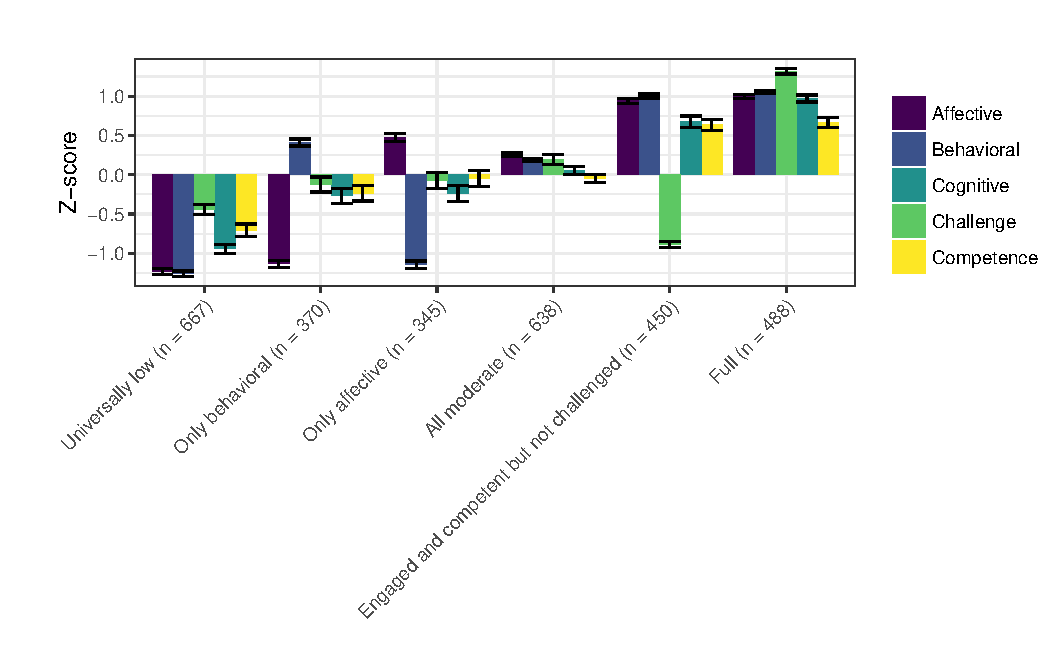
\includegraphics[width=1\linewidth]{rosenberg-dissertation_files/figure-latex/unnamed-chunk-11-1} 

}

\caption{The six profiles of engagement (with variable values standardized)}\label{fig:unnamed-chunk-11}
\end{figure}

\begin{figure}

{\centering 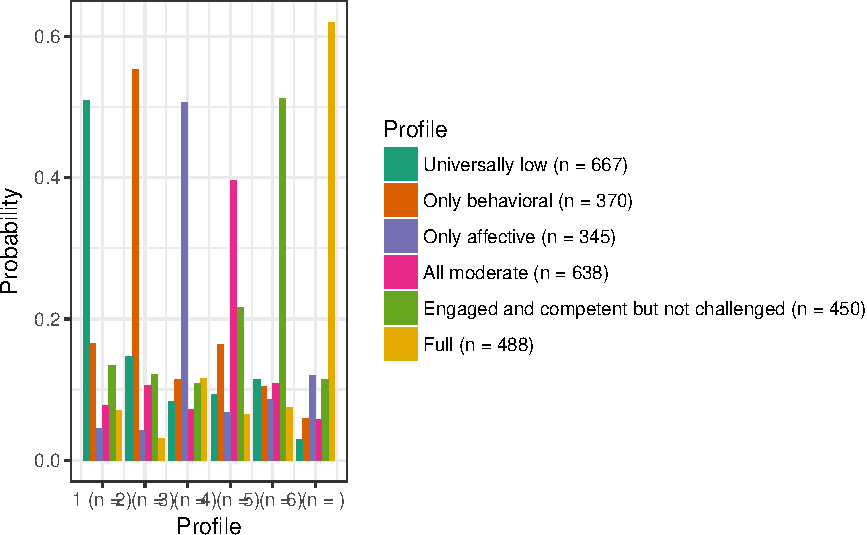
\includegraphics[width=0.8\linewidth]{rosenberg-dissertation_files/figure-latex/unnamed-chunk-12-1} 

}

\caption{The six profiles of engagement (with raw variable values)}\label{fig:unnamed-chunk-12}
\end{figure}

This solution is characterized by:

\begin{itemize}
\tightlist
\item
  A \emph{universally low} profile, characterized by low levels of
  working hard, learning something new, and enjoying the activity, and
  perceptions challenge and competence
\item
  An \emph{only behaviorally engaged} profile, with moderate levels of
  working hard, very low enjoyment of the activity, and moderately (low)
  levels of learning something new and challenge and competence
\item
  An \emph{only affectively engaged} profile, with moderate levels of
  enjoyment, low levels of hard work, and moderately (low) levels of
  cognitive learning something new, challenge, and competence
\item
  An \emph{all moderate} profile, with moderate levels of the three
  indicators of working hard, learning something new, enjoying the
  activity, challenge, and competence
\item
  An \emph{engaged and competent but not challenged} profile,
  characterized by high levels of working hard, learning something new,
  enjoying the activity, and competence, but with low levels of
  challenge
\item
  A \emph{full} profile, with high levels of working hard, learning
  something new, enjoying the activity, challenge, and competence
\end{itemize}

The six profiles are characterized by both varying levels on both the
indicators of engagement (cognitive, behavioral, and affective) and
perceptions of challenge and competence. Also, the number of
observations across the profiles is relatively balanced (with no
profiles associated with a very large or small number of observations).
The universally low profile was associated with the most substantial
number of observations (\emph{n} = 667), followed by the all moderate
profile (\emph{n} = 638); each of the other four profiles was associated
with 300 to 400 observations. The results for research questions 3-5 use
this solution and the six profiles in subsequent analyses.

\section{Results for Research Question \#3: What sources of variability
are there for the profiles of
engagement?}\label{results-for-research-question-3-what-sources-of-variability-are-there-for-the-profiles-of-engagement}

For all six profiles, the \emph{ICC}s (for the model with only the
youth, instructional episode, and program levels themselves, but not
variables at the levels) represent the systematic variability (the
proportion of variance explained) associated with each of the levels for
each profile. Thus, the different levels can have different proportions
of variance explained for different profiles. The systematic variability
at the youth level, for example, could be .10 for the \emph{Full}
profile and .025 for the \emph{Universally Low} profile. At the program
level, the \emph{ICC}s were found to be small, with values ranging from
0.00 to 0.023, suggesting that little variability can be explained by
the program. For the instructional episode level, the \emph{ICC}s were
also small, ranging from 0.004 to 0.01. Finally, at the youth level, the
\emph{ICC}s ranged from .093 to .432.

\begin{table}

\caption{\label{tab:unnamed-chunk-13}Intra-class correlation (ICC) values for each of the three levels}
\centering
\begin{tabular}[t]{lrrr}
\toprule
Profile & Instructional Episode & Youth & Program\\
\midrule
Universally low (n = 667) & 0.006 & 0.267 & 0.023\\
Only behavioral (n = 370) & 0.006 & 0.093 & 0.009\\
Only affective (n = 345) & 0.004 & 0.262 & 0.003\\
All moderate (n = 638) & 0.015 & 0.310 & 0.000\\
Engaged and competent but not challenged (n = 450) & 0.009 & 0.100 & 0.000\\
Full (n = 488) & 0.031 & 0.432 & 0.019\\
\bottomrule
\end{tabular}
\end{table}

In terms of **ICC\emph{s at youth level across the six profiles, the
value for the youth-level ICC was highest for the }Full* profile
(\emph{ICC} = .432), suggesting that some youth have a strong tendency
to be fully engaged (possibly due to their initial interest or other
individual characteristics and differences). The other profile
characterized by a consistent pattern across all of the variables--the
\emph{Universally low} profile--had a modest value for the ICC at the
youth level (\emph{ICC} = .267). Finally, a significant amount of
variability is associated with the residual (variance that is not
associated with the program, instructional episode, or youth levels).
This suggests that there is wide variation in youths' responses that may
not be readily explained or predicted by variables \emph{at one level
alone}. Remaining unexplained variability is captured by the residual
term. Some youth from particular programs may engage during some episode
instructional episodes in very high or low ways that are not captured by
modeling the variability at each of these levels alone.

The \emph{ICC}s lend insight into the sources of variability for a
specific profile; within-youth stability in terms of how frequently they
reported particular profiles could lend further insight by considering
variability across profiles. This analysis can be particularly useful
for understanding variability at the youth level, which the \emph{ICC}s
show to be associated with the most systematic variability. Each youth
has a most-frequently reported profile. Results show that for some
youth, the profile is very dominant, occurring in a substantial
proportion of youths' responses; for others, it occurs not that
frequently, meaning that youth report a variety of different profiles.
As presented in Figure 4.3, the mean proportion of responses for each
youth in the profile they reported most varied widely across youth.
Specifically, on average, youth reported their most-reported profile in
.540 (\emph{SD} = .194, \emph{min} = .182, \emph{max} = 1.00) of their
responses. There was a small number of youth who reported the same
profile in all of their responses, but for most youth, the profile they
reported most made up only a portion of all of their responses. For most
youth, the most common profile was observed just over 50\% of the time.

In sum, these findings show that there was substantial variability in
the profiles present at the youth level. Less variability was explained
by either the program youth were in or the nature of the particular
instructional episode present when youth were signaled. These results
set the stage for those for the next two research questions, on the
relations between the aspects of work with data (for research question
\#4) and the youth characteristics (for research question \#5) and the
profiles of engagement.

\begin{figure}

{\centering 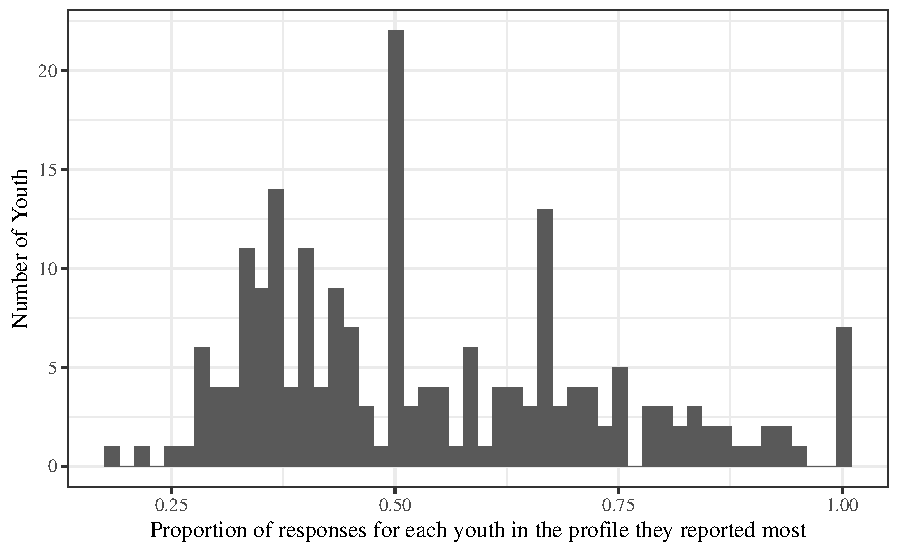
\includegraphics[width=0.8\linewidth]{rosenberg-dissertation_files/figure-latex/unnamed-chunk-14-1} 

}

\caption{Histogram of the proportion of responses for each youth in the profile they reported most}\label{fig:unnamed-chunk-14}
\end{figure}

\section{Results for Research Question \#4: Aspects of work with data
and
engagement}\label{results-for-research-question-4-aspects-of-work-with-data-and-engagement}

To understand how aspects of work with data are related to engagement,
six analytic models were specified -- one for each engagement profile.
In each model, the dependent variable is the probability of a response
being classified in a particular profile (for example ``fully
engaged''), as determined by the Latent Profile Analysis. The five
aspects of work with data were the predictor (or independent) variables.
Because various aspects of work with data tended to co-occur,
simultaneously entering indicators for all five aspects isolates the
association for any single aspect while controlling on the presence of
the others. All models also include some youth characteristics which
will be used to answer research question five below.

Associations between the five aspects of work with data and the six
engagement profiles are presented in Table 4.5. In this table, each
column represents the output from one of the six different models. As an
example, the first column reports the coefficients for the associations
between the predictor variables and the \emph{Only behavioral} profile.
Because the outcome is in the form of a probability (ranging from 0.00
to 1.00), it can be interpreted as the change in the probability of a
response being associated with each profile. Note that the
\emph{p}-values are calculated using the most conservative and
recommended by recent research Kenward-Rogers approximation (Halekoh \&
Hojsgaard, 2014).

The only engagement profile that was significantly associated with any
aspects of work with data was the Full profile (see the column with the
column name Full for these results). When program activities involved
modeling data, youth were around 3\% more likely to be fully engaged
(\(\beta\) = 0.034 (0.017), \emph{p} = .020; partial \(R^2\) = .002). In
other words, when program activities included modeling data, youth are
more likely to report working harder, learning more, enjoying themselves
more, and feeling more competent and challenged.

Youth were also more likely to be in the Full engagement profile when
program activities included generating data (\(\beta\) = 0.027 (0.015),
\emph{p} = .033; partial \(R^2\) = .002). These particular program
activities increased the probability of full engagement by around 3\%.
To sum up these two findings, modeling data and generating data are
associated with a (very) positive form of engagement, that exhibited by
the Full profile. However, the effect sizes indicate quite small effects
in substantive terms.

Sensitivity analysis was carried out for the statistically significant
two effects was carried out to determine just how robust they were. This
follow-up analysis revealed that the effect of modeling data on
\emph{Full} engagement much more robust than that for generating data:
9.835\% of this effect (of data modeling) would have to be due to bias
to invalidate the inference about its effect. For generating data, only
1.884\% of the effect of generating data would need to be due to bias to
invalidate the inference about its effect. These values are not
minuscule but are also not very large (Frank, 2003). So, while
statistically significant, the effect of data modeling seems to be a
more robust effect than the effect of generating data, which does not
seem to be a very robust (and should, therefore, be interpreted with
some caution).

\begin{verbatim}
## Error in inherits(x, "list"): argument "x" is missing, with no default
##               [,1]              [,2]              [,3]            
## Profile       "Universally low" "Only behavioral" "Only affective"
## Pre-interest  "-0.047 (0.022)"  "-0.013 (0.012)"  "-0.012 (0.019)"
## Gender-Female "0.06 (0.037)+"   "0.019 (0.019)"   "-0.038 (0.033)"
## URM status    "-0.01 (0.052)"   "0.031 (0.026)"   "-0.076 (0.046)"
## Asking        "-0.015 (0.018)"  "0.015 (0.015)"   "0.023 (0.017)+"
## Observing     "0.003 (0.018)"   "0.013 (0.015)"   "0.007 (0.017)" 
## Generating    "-0.014 (0.017)"  "0.014 (0.014)"   "0.012 (0.016)" 
## Modeling      "0.004 (0.019)"   "-0.023 (0.016)"  "-0.004 (0.018)"
## Communicating "0.002 (0.018)"   "0.018 (0.015)"   "-0.011 (0.017)"
##               [,4]                            [,5]            
## Profile       "Eng. and comp. but not chall." "All moderate"  
## Pre-interest  "0.039 (0.016)*"                "0.007 (0.01)"  
## Gender-Female "0.025 (0.028)"                 "-0.02 (0.018)" 
## URM status    "-0.012 (0.04)"                 "0.018 (0.025)" 
## Asking        "-0.011 (0.015)"                "0.004 (0.014)" 
## Observing     "0.009 (0.015)"                 "-0.017 (0.014)"
## Generating    "-0.014 (0.014)"                "-0.02 (0.013)" 
## Modeling      "0 (0.015)"                     "-0.012 (0.015)"
## Communicating "0.004 (0.015)"                 "0.016 (0.014)" 
##               [,6]            
## Profile       "Full"          
## Pre-interest  "0.018 (0.021)" 
## Gender-Female "-0.035 (0.037)"
## URM status    "0.043 (0.053)" 
## Asking        "-0.019 (0.016)"
## Observing     "-0.025 (0.016)"
## Generating    "0.027 (0.015)*"
## Modeling      "0.034 (0.017)*"
## Communicating "-0.027 (0.016)"
\end{verbatim}

\section{Results for Research Question \#5: Youth characteristics and
engagement}\label{results-for-research-question-5-youth-characteristics-and-engagement}

Associations between youth characteristics and the six profiles are
reported in the top half of Table 4.5. Youth who enter the program with
higher levels of interest (in STEM) are more likely to report being in
the engaged and competent but not challenged profile (\(\beta\) = 0.039,
\emph{p} = .009; partial \(R^2\) = .001). In other words, youth who are
more interested at the outset of the program report working harder,
learning more, enjoying themselves more, and feeling more competent when
they are involved in program activities, though they also report lower
levels of challenge. For this effect, 17.879\% would be needed to
invalidate the inference, suggesting a moderately robust effect.

In terms of youths' pre-program interest, these analyses show that youth
who enter the program with higher levels of interest (in STEM) are more
likely to report being in the \emph{Engaged and competent but not
challenged} profile (\(\beta\) = 0.039, \emph{p} = .009; \emph{partial
\(R^2\)} = .001). For each one-unit increase in pre-program interest in
STEM, youth are around 4\% more likely to report this profile. In other
words, youth who are more interested at the outset of the program report
working harder, learning more, enjoying themselves more, and feeling
more competent when they are involved in a program's activities, though
they also report lower levels of challenge. For this effect, 17.879\%
would be needed to invalidate the inference, a slightly larger value for
the follow-up sensitivity analysis than those found for the
(statistically significant) relations involving the aspects of work with
data, suggesting a moderately robust effect.

There were not any statistically significant effects of youths' URM
status. This may be a function of the large proportion of youth from
under-represented (in STEM) racial and ethnic groups. Hispanic (48\%),
African American or Black (36\%), and youth who identify as being from
multiple racial and ethnic groups (3\%) made up 87\% of the youth in the
programs, so there were not many youth \emph{not} from under-represented
groups in the sample, suggesting that the absence of findings may be due
to this small sample (and low statistical power). Nevertheless, no
relations between URM status and youths' engagement were found,
indicating that there is at least no evidence that youth from such
backgrounds do engage in different ways.

These (somewhat minimal) findings for the youth characteristics were
more surprising than those observed for the aspects of work with data.
The results of research question \#3, on the sources of variability for
the profiles of engagement, suggested that there was much systematic
variability at the level of the youth (there were large \emph{ICC}s at
the youth level, with smaller \emph{ICC}s at the instructional episode
level). Because pre-interest, gender, and URM status are variables at
this level, it could be expected that they would have meaningful
relations with the profiles of engagement. However, it appears that the
particular youth characteristics considered were not useful at
explaining much of this variability; possible reasons why are discussed
further in the next section.

\chapter{Discussion}\label{discussion}

Each of the disciplines that contribute to STEM learning - science,
technology and computer science, engineering, and mathematics - involve
work with data. While past research has focused on what aspects of work
with data learners are involved in with respect to work with data, or
specific conceptual outcomes from working with data, little research has
considered youths' engagement when they work with data. In this study,
engagement was used as a lens to understand the experience of youth
working with data during summer STEM programs. In particular, five
aspects of work with data, a) asking questions, b) observing phenomena,
c) constructing measures and generating data, d) data modeling, and e)
interpreting and communicating findings, were identified from
video-recordings of the programs. The nature and frequency of these
codes was explored, and then the codes were used to predict, along with
youths' characteristics, profiles of engagement. These profiles of
engagement depict distinct groups on the basis of different levels, of
youths' cognitive, behavioral, and affective engagement, and youths'
perceptions of challenge and competence.

Findings indicate that work with data occurs frequently in the programs
and that there are some examples of ambitious activities centered on
working with real-world data as well as some that highlight the
heterogeneity in how work with data is enacted in them. Six profiles of
engagement were identified, representing different configurations of
engagement. Relations of work with data and youth characteristics
(pre-program interest in STEM and youths' gender and status in terms of
being a member of under-represented groups in STEM) were, overall, not
strongly related with the profiles of engagement, though some key
findings were identified. Generating and modeling data were both related
to the most potentially beneficial profile, one characterized by high
levels of all five of the variables used to create the profiles. This
study suggests that work with data has affordances in terms of
understanding the nature of what youth do in summer STEM programs. These
findings also show the value of an innovative method, ESM, and a
modeling approach designed to identify engagement in a holistic manner,
LPA, that together provide some access to youths' experience
in-the-moment of the activities they were involved in during the
program. Data, and who is able to work with it, important roles in STEM
learning and in society; efforts to understand and support learners
engaging in these ambitious activities should be encouraged and
expanded.

\section{Key findings related to work with data in summer STEM
programs}\label{key-findings-related-to-work-with-data-in-summer-stem-programs}

Work with data was common in the summer STEM programs. 170 out of the
236 instructional episodes contained at least one of the five aspects
(asking questions, making observations, generating data, data modeling,
and interpreting and communicating findings) of work with data. The use
of video-recordings of the programs and the strategy of using ESM to
select (mostly) random samples of youths' experiences during the
programs enabled me to show just how frequent work with data was, and I
found that specific aspects of work with data were more or less
frequent: Making observations, in some form, occurred during 24\% of the
program's time, for example, while generating data and communicating
findings both occurred more frequently, during 43\% of the instructional
episodes. These findings, broadly, suggest that work with data occurred
enough that we might expect to see differences in youths' engagement.

Given the design and goals of summer STEM programs, these align with
what may be expected given past research: Such programs are designed to
engage youth in the practices, including and as I argue earlier
\emph{especially} those relating to work with data, of STEM domains
(Dabney et al., 2012; Elam et al., 2012). Even still, these are the
first results of this kind (in terms of the proportion of the time spent
in the programs). Using video-recording data and a sampling strategy
that can provide insight into the amount of overall time spent was an
important component of achieving these findings. While there are not
other results of this particular kind, a related, an area of related
work concerns other studies that have used the PQA measure. However,
studies have (yet) used the version that is adapted for STEM content
areas. Some reports call for greater use of measures (such as the PQA)
in the study (and evaluation) of summer and outside-of-school STEM
programs (e.g., Yohalem et al., 2005). As one example of such a study
(but one that is not focused on STEM), Smith et al. (2012) reported
findings from a continuous improvement intervention (that used a
rigorous experimental design), finding that the intervention positively
impacted the quality of instruction in the programs.

In addition to work with data being common, it was highly varied in
nature. In-depth qualitative analysis revealed that there was often a
variety of ways in which each of the aspects were carried out, with
implications for how youth may engage in each of them. Many times, youth
engaged in what can be described as ambitious and potentially highly
engaging ways of being involved in work with data. When youth were
asking questions, 39\% of the time they worked to make predictions or
hypotheses about the phenomena they were exploring or the problem they
were seeking to solve. When making observations, in 86\% of the
episodes, they did so of phenomena in the field (such as an estuary or
an island in the case of science-focused programs). In mathematics and
engineering-focused programs, such observations were of the physical
objects that youth created in workshops or were through computers in
classroom settings. These findings suggest, broadly, that there were
opportunities available for youth to be highly engaged in work with
data.

When generating data, many times (in 47\% of the episodes that involved
this aspect) youth recorded their own observations; when modeling data,
youth were involved (in 72\% of the episodes) in the use of statistical
and mathematical models of real-world phenomena. When interpreting and
communicating findings, youth regularly (during 48\% of episodes) had
opportunities to share (with other youth in the program) what they found
or created as a result of their earlier investigations or work. Also of
note was what occurred during the rest of the time: When youths'
questions, for example, were not focused on predicting or hypothesizing
about what they were exploring, type of question was more general, or
was instructor-led, rather than driven by youth, forms of work with data
that is much more variable than may be expect by recent reform efforts
(i.e., National Research Council, 2012; NGSS Lead States, 2013; National
Governors Association Center for Best Practices, Council of Chief State
School Officers, 2010), but more expected given past research pointing
out variability in what evidence and data mean, especially in science
education settings (McNeill and Berland, 2017; Lehrer \& Schauble,
2015).

Also of note was the frequency of these three aspects of work with data
overall: They occurred much more frequently than the two (making
observations and data modeling) for which a larger proportion of their
enactment was more in-line with policy and curricular standards. The
type of activities that may be the most demanding for youth were still
common, but not quite as common as the overall frequencies presented for
the quantitative would suggest.

While descriptive in nature, these results present the first insight
into the extent of work with data in STEM enrichment programs. They
suggest that, as past scholarship (National Research Council, 2009,
2012) can provide a context for youth to be involved in the type of
scientific and engineering practices-focused activities that can be
particularly powerful for youth (and students) in terms of their
learning. The use of video-recordings of data was especially helpful in
establishing this descriptive data.

Past research does point out the heterogeneity in how work with data is
enacted in educational settings. Past research, for example, highlights
use of ``data to solve real problems and to ask authentic questions''
(Hancock et al., 1992, p.~337). Research on generating data emphasized
an aspect not very much the focus of the present research, namely,
structuring data into spreadsheets (Konold, Finzer, \& Kreetong, 2017;
Lehrer \& Kim, 2009). Research on posing questions that can be answered
with data shows that there is a connection between student-centered
teaching strategies and students' ability to ask empirical (Bielik \&
Yarden, 2016). This suggests a reason why youth were able to ask
questions and ideas for how they might do so more: Make activities in
summer STEM program youth-centered, rather than instructor-centered.
Research on the data modeling aspect of work with data highlights the
use of statistical models much more than the physical models which were
sometimes found to be a way in which youth engaged in data modeling
(Petrosino, Lehrer, \& Schauble, 2003; Lesh, Middleton, Caylor, \&
Gupta, 2008; Lee, Angotti, \& Tarr, 2010). Nevertheless, many of the
ways youth engaged in data modeling aligned with this past research,
particularly when the goal of the activity is to model variability. This
past research that encouraging youth to consider summaries of data, such
as the mean and standard deviation, may be a promising way for them to
engage more deeply in data modeling (Lehrer, Kim, \& Schauble, 2007;
Lehrer \& Schauble, 2004). In this way, some (but not all) of the
aspects work with data aligned with past research; when they align, they
are encouraging, and when they do not, some ideas for how to involve
youth in more engaging aspects of work with data are able to be
identified.

\section{Key findings related to
engagement}\label{key-findings-related-to-engagement}

Six profiles of engagement were found using a rigorous model selection
approach. Before discussing these results in-depth, it is important to
note that LPA is an exploratory approach: The number and nature of the
profiles identified were found through a rigorous and systematic
approach, but this is not a guarantee that the same number and make-up
of profiles would emerge in other samples and other contexts: These
profiles should be considered as initial evidence, and not as proof that
these are \emph{the} six profiles of engagement that will exist in all
settings.

The number of profiles found is broadly similar to that found in past
research. Six profiles is the same number of profiles of engagement
identified in recent, past research and the similar number provides
further information about the nature of engagement in educational
contexts: Schmidt et al. (2018) found six profiles of engagement. Their
profiles were constructed on the basis of the indicators (cognitive,
behavioral, and affective) of engagement, and not perceptions of
challenge and competence. As Schmidt et al.`s study is the only other to
examine engagement profiles, another point of comparison is other,
similar outcomes, including youths' (and students') motivation (see
Wormington and Linnenbrink-Garcia, 2017, for a review in motivational
settings). Wormington and Linnenbrink-Garcia (2017) report that,
usually, a smaller number, with only two of the 22 studies reviewed
finding six profiles. This suggests, on the basis of this study and
Schmidt et al.'s (2018) study, that there may be a greater variety of
types of engagement exhibited than, for example, types of motivation.

In terms of the make-up of the specific profiles, those found in the
present study included those that were strongly negative
(\emph{Universally low}) and strongly positive (\emph{Full}), as well as
those characterized by different levels of engagement (\emph{Only
behavioral} and \emph{Only affective}) and by different levels of the
conditions of engagement (Engaged and Competent but not Challenged). An
\emph{All moderate} profile was also identified. Little research has
examined profiles of engagement, though Schmidt et al. (2018) examined
profiles of engagement, constructed from items for cognitive,
behavioral, and affective engagement (but not perceptions of challenge
and competence), and found six profiles, some of which partially overlap
with those found in the present study. In particular, on the basis of
the items shared between the studies, a \emph{Universally low},
\emph{All moderate}, and \emph{Full} profile were found in both studies.
However, as these profiles are characterized by the (uniform) level
across all of the variables, this is only limited evidence for the
presence of these profiles in the larger population of youth engaged in
science and STEM-related learning activities.

These profiles have implications for the study of engagement and the
analysis of multidimensional data on youth and student engagement.
First, they suggest that perceptions of challenge and competence be
considered in future research. This is because some of the profiles were
distinguished on their basis. This approach also may be more
parsimonious than including perceptions of challenge and competence as
separate predictors (i.e., Shernoff et al., 2003). In addition to these
empirical reasons, past research on engagement (i.e., Csikszentmihalyi,
1990) and on the profile approach (Bergman \& Magnusson, 1997) suggest
that they are theoretically inseparable from engagement, another reason
for modeling them as they were modeled in the present study. These
implications are specific to the study of engagement but also highlight
some of the promise of the profile approach, as well.

\section{Key findings related to work with data and youth
characteristics and their relations to
engagement}\label{key-findings-related-to-work-with-data-and-youth-characteristics-and-their-relations-to-engagement}

The source of variation in the profiles of engagement that \emph{can be}
explained can be due to many different factors, including individual
differences between youth, the nature of the instruction carried out,
and program-specific factors. Knowing about these sources provide
valuable information in their own right, a benefit of the use of mixed
effects models (Gelman \& Hill, 2007). First, this study explored the
sources of variability for the profiles of engagement, revealing that
little variability was at the instructional episode level (important
given that work with data is a variable at this level) and at the
program level. This suggests that engagement, as measured in this
context with ESM and with the engagement items used, may be more stable
than dynamic at the instructional episode level, differing from some
past theory (e.g., Skinner \& Pitzer, 2012) and research that showed
relations between instructional episode-level variables and engagement
(e.g., Shernoff et al., 2016; Shumow, Schmidt, \& Zaleski, 2013). This
also suggests that variables at these levels do not have a substantial
proportion of variability to explain: Predictor variables (like those
for the aspects of work with data) at the instructional episode level
had much less variability to explain, while those at the youth level had
a substantial amount that was able to be explained.

In line with what the sources of variability would suggest, relations
between work with data were largely not found, though some small,
statistically significant relations were identified. These findings,
overall, were not necessarily surprising given past research: The
question of whether and how work with data relates to engagement has not
been the focus of any past research. In this sense, these are important
findings that suggest that work with data may not be strongly related to
engagement.

Given the small amount of variability at the instructional episode
level, this result was anticipated (on this basis). Importantly,
however, there were some noteworthy findings. In particular, both
generating and modeling data were found to be positively (and
statistically significantly) related to the \emph{Full} profile,
suggesting that when youth are involved in these practices, then they
are more likely to be highly engaged. In particular, given the makeup of
this profile, this suggests that when youth are involved in these
aspects of work with data, they are more likely to report high levels of
cognitive, behavioral, and affective engagement, and high perceptions of
competence and challenge. Generating and modeling data may have such
relations because they are particularly important aspects of work with
data. As Lehrer and Schauble (2006) explain, \emph{inscriptions serve
commitments}: Choosing to record an observation or an idea as data
involves the process of identifying something that is worth recording
and then recording the parts that are of interest. Thus, generating data
may be fully engaging to youth because it is, generally, demanding and
important with respect to work with data. Modeling, too, is an important
practice. It been described as \emph{the} central scientific and
engineering practice (Schwarz et al., 2009; Lehrer \& Schauble, 2015;
Weisberg, 2012), and its relations with full engagement provides some
actionable evidence for its importance in the context of summer STEM
programs.

As there is no research on how work with data relates to youths'
engagement, the findings associated with this research question provide
some (albeit limited) evidence, and directions for future research for
how some aspects of work with data relate to youths' engagement. As work
with data is a core component of new visions for STEM learning (see the
scientific and engineering practices that are part of the NGSS and the
standards for mathematical practice in the CCSS), these findings provide
some insight into how involvement in a subset (focused on work with
data) of these practices relates to engagement. Particularly, the
relatively minimal findings suggest that these activities may not be
more engaging \emph{per se}. Instead, it may be the way that youth
engage in them that matters, in alignment with past research (Berland et
al., 2017; Miller et al., in press).

While the findings for this question were somewhat minimal, there are
key findings from both the important relationships that were found to be
statistically significant (between generating data and data modeling and
\emph{Full} engagement) and from those that were not. Finding few
significant findings may show that, in this sample and with work with
data as carried out, it is difficult to say with certainty just how much
of an impact work with data has upon youths' engagement. This suggests
that other samples, other enactments of work with data, and, possibly,
other analytic approaches can build on this work to further substantiate
what is known about how work with data is engaging to youth.

The relations between youth characteristics and the profiles were found
to be small and not as much in line with expectations given the
preliminary analysis. These small relations were similar (in magnitude)
to those between work with data and the profiles, but they were more
surprising for a reason related to the sample for this study, namely,
given the substantial variability at the youth level among the
responses. This is described in detail in the discussion of the findings
for research question \#3.

There was a lot of variability in the profiles of engagement at the
youth level, but not many relations. Findings revealed that youth with
higher pre-program interest were more likely to be \emph{Engaged and
competent but not challenged}. This suggests that youth with higher
interest in STEM are inclined to be highly engaged and good at what they
are doing, but are not challenged by the activities they experience.
This finding is in line with past research suggesting a relationship
(direct or as a moderator) between youth characteristics (including
interest) and their engagement (Shernoff et al., 2003; Shernoff et al.,
2016; Strati et al., 2017). More specifically, this finding suggests
that for youth who are particularly interested (and those who choose to
attend) summer STEM programs, what they are involved in may not
challenge them very highly. This finding has implications for past
research that shows youth who choose to attend summer STEM programs are
more engaged (but that does not speak to their degree of challenge;
Beymer, Rosenberg, Schmidt, \& Naftzger, 2018).

While the findings for this research question, like those for the
relations between the aspects of work with data and youths' engagement,
they provide some information about how these characteristics relate to
youths' engagement. Finding that youth who are more interested prior to
the beginning of the summer STEM programs are more likely to be working
hard, learning something new, and enjoying what they are learning, and
perceive themselves to be good at what they are doing but not
challenged, is a meaningful finding. Moreover, the null findings suggest
that other characteristics, including those measured but not included
for this analysis (such as youths' pre-program perceptions of their
competence) as well as those not measured at all, may be considered in
follow-up studies and in future research.

Why might these findings be so limited? One reason may be that summer
STEM programs are different from other contexts in terms of work with
data: While the programs that were involved in the study have many
affordances for work with data and for being highly engaging for youth,
they have some limitations, too, particularly with respect to support
work with data. Importantly, these were not programs explicitly designed
to support work with data; while such contexts are being developed, they
are not yet widespread. Moreover, youth may perceive the programs to
have lower stakes in terms of their future. This may mean that the
individual activities that youth engage in is less connected to their
engagement: Youth instead engage in typical (to each youth) ways, rather
than in ways that are much more sensitive to changes in their context.
Another possible explanation for these limited findings may be that
youth are not very challenged or are not very supported: A profile with
low challenge but high competence and cognitive, behavioral, and
affective engagement was found, suggesting that youth may be engaged and
good at what they are doing, but are not challenged: Greater challenge
may be found to be associated with more full engagement.

Learning environments that deliberately support work with data over a
long period may demonstrate different patterns of engagement than those
examined in this study because of the focus on and sequencing of the
aspects of work with data, which may make it more (or less) cognitively,
behaviorally, or affectively engaging than is determined in this study.
As Miller et al. (2018) highlight, truly engaging STEM activities are
not easily come by; they require students to take ownership over and to
make decisions about their explorations or designs. Thus, future
research may study work with data in contexts designed to support it. A
key part of this future research may be studying both work with data and
how work with data is supported (most importantly by the instructor but
also by the curriculum and technological tools).

\chapter{Limitations to the present study and recommendations for
research}\label{limitations-to-the-present-study-and-recommendations-for-research}

This study examines youths' engagement as an outcome. Accordingly,
outcomes from engaging, such as the products of neither youths' work or
the specific cognitive capabilities they develop through their
participation, are not the focus. Thus, while some findings about how
work with data and youth characteristics were found to be associated
with different profiles of engagement, we do not have an understanding
of how engaging in more or less adaptive ways relates to these outcomes.
Examining how work with data and engagement relate to key learning,
motivational, and future goals and plans-related outcomes is a topic for
future research.

It is possible that the somewhat minimal findings are, in part, a result
of the analytic approach. A similar mixed effects modeling approach has
only been used in one other study (Strati et al., 2017), and that
approach did not use profiles (as in this study) as the outcome. In this
study, little variability at the instructional episode level was found,
and so minimal relations between factors at this (instructional episode)
level and the profiles of engagement was expected. Might profiles, but
not the variables used to create them, be less variable at the
instructional episode level? One way to consider such an alternate
explanation is to use the data used in this study as part of a
correlational analysis, or another analysis that uses that variables
used to create profiles of engagement but does not use the profiles
themselves.

There were some general measurement-related limitations. Work with data
can be difficult to measure because, as the qualitative analysis
revealed, there are a variety of ways in which youth can be involved in
work with data. Related,, work with data was measured as being present
or not present; might a scale, that measures gradations of work with
data, or a learning progression for work with data, be used as part of
different measures? More specific in terms of the alignment of the
measure with the conceptual framework for work with data, the dimensions
of the STEM-PQA measure aligned closely with the aspects of work with
data. But, there were some possible divergences that may have had an
impact upon some of the findings. For example, for the interpreting and
communicating findings code, the STEM-PQA codes for \emph{Analyze}
(``Staff support youth in analyzing data to draw conclusions'') and
\emph{Use symbols or models} (``Staff support youth in conveying STEM
concepts through symbols, models, or other nonverbal language'') were
used. In the case of the latter STEM-PQA code, conveying STEM concepts
through symbols, models, or other nonverbal language could have
reflected instructional episodes in which youth used, for example,
mathematical equations or formulas, but did not do so as part of
modeling data of a phenomena in the world: They could have simply been
using an equation outside of the context of any particular phenomena.
Future research may consider use of coding for this aspect of work with
data (and this aspect of science curricular standards in particular; see
NGSS Lead States, 2013).

As another example of this limitation, generating data was an aspect of
work with data that the open-ended qualitative analysis revealed to be
less associated with less systematic groups of practices, or themes,
than the other aspects. The STEM-PQA codes corresponding to this aspect
of work with data were \emph{Collect data or measure} (``Staff support
youth in collecting data or measuring'') and \emph{Highlight precision
and accuracy} (``Staff highlight value of precision and accuracy in
measuring, observing, recording, or calculating''). Particularly in the
case of the latter code, the emphasis on precision and accuracy may have
been outside of activities focused on recording data or creating coding
frames. Future research may consider a coding frame that is (even more)
focused on generating data, though considerations of precision and
accuracy are key aspects of doing so, and so perhaps separating the act
of generating data from considerations that are important to keep in
mind while doing it may be a promising direction for future research.

While these divergences in measures were not large, they suggest that
the coding frame for work with data is a limitation of the present
study. McNeill and Berland (2017) describe a similar type of
disagreement across science education settings: While a limitation, the
coding frame did represent agreement across a range of studies across
STEM contexts for the aspects of work with data, although I recognize
that this coding frame may not distinguish the different ways in which
work with data is enacted, as revealed by the qualitative coding carried
out in this study.

One factor of note concerns the analytic approach used. As noted, the
profiles demonstrated very little variability at the program and
instructional episode level, suggesting that factors at this level would
likely not strongly predict the profiles. This could be a function of
the use of profiles and the specific variables selected. It may also be
the result of the outcome (engagement and its conditions) selected.
Other analytic approaches can be carried out to determine the viability
of the profiles approach and use of the items for engagement and its
conditions for understanding work with data.

While these are important limitations, it is worth noting that the
modeling strategy (with the mixed effects models) is inherently a
conservative (particularly in terms of the statistical significance of
hypothesis tests) approach. Thus, while the findings detected are small,
they can be considered to be trustworthy on the basis of the way the ESM
data were analyzed. This trustworthiness is enhanced by the use of
sensitivity analysis, which showed how much of the effects could be due
to bias for them to be invalidated.

For example, as McNeill and Berland (2017) argue, it is not just
engaging in these practices by rote, but about integrating them, as they
overlap and interconnect.They argue that a view of work with data
focused on sense-making with real-world phenomena and iterative cycles
of engaging in work with data, and revision of intermediate ideas.

\chapter{Implications for Practice}\label{implications-for-practice}

Two key implications related to engaging youth in generating and
modeling data and including other practices to the extent that they
involve youth in generating and modeling are discussed. This is based on
the increases in full engagement when youth are involved in these
activities, all else being equal. While this is somewhat limited
evidence, this study suggests that \emph{generating data} and
\emph{modeling data} in particular may be beneficial in terms of
engaging youth.

Practically, youth activity leaders (in summer STEM and other STEM
enrichment contexts) and teachers (in formal learning environments) can
best include the beneficial practices of generating and modeling data
not in isolation, but rather through involving youth and learners in
complete cycles of investigation. This aligns with both foundational and
contemporary research on work with data in education (Berland et al.,
2018; McNeill \& Berland, 2017; Hancock et al., 1992; Lee \& Wilkerson,
2018). Recent curricular reform efforts also suggest that the best way
to engage learners in particular practices is through the process of
identifying a question or problem, marshaling sources of data that can
be used to figure out what is happening, and developing model-based
explanations that are then communicated (or even used in an argument;
National Governors Association, 2013; National Research Council, 2012;
NGSS Lead States, 2013). With respect to work with data in particular,
youth activity leaders and teachers can use the findings from this study
as a starting point to consider how engaging in work with data may also
prepare learners to think of, understand, and take action based on data
in their day-to-day lives. Many questions or problems learners face may
involve data that can be meaningfully incorporated into engaging
learning activities.

A final note concerns how the modeling was carried out. Because LPA is
an exploratory approach, it requires a blend of exploring the data while
also systematically taking account of how the solutions change while
different solutions are explored. Because of the challenge of doing
this, I developed an open-source tool that made it easier to work toward
the aim of systematically exploring the data. Other educational
researchers may consider the utility of such development efforts, though
such efforts are not a regular part of the products created in the
course of most educational research. Such development work by
educational researchers may even inform the type of activities youth do
when working with data: While a STEM content area, programming and
computer science-related activities were not emphasized as much as those
related to science, mathematics, and engineering.

\chapter{References}\label{references}

\setlength{\parindent}{-0.2in} \setlength{\leftskip}{0.2in}
\setlength{\parskip}{8pt} \noindent

Akiva, T. (2005). Turning training into results: The new youth program
quality assessment. High/Scope Resource, 24(2), 21-24.

Bergman, L. R., \& Magnusson, D. (1997). A person-oriented approach in
research on developmental psychopathology. Development and
psychopathology, 9(2), 291-319.

Bergman, L. R., Magnusson, D., \& El Khouri, B. M. (2003). Studying
individual development in an interindividual context: A person-oriented
approach. Psychology Press.

Berland, L. K., Schwarz, C. V., Krist, C., Kenyon, L., Lo, A. S., \&
Reiser, B. J. (2016). Epistemologies in practice: Making scientific
practices meaningful for students. Journal of Research in Science
Teaching, 53(7), 1082-1112.

Bielik, T., \& Yarden, A. (2016). Promoting the asking of research
questions in a high-school biotechnology inquiry-oriented program.
International Journal of STEM Education, 3(1), 15.

Breckenridge, J. N. (2000). Validating cluster analysis: Consistent
replication and symmetry. Multivariate Behavioral Research, 35(2),
261-285.

Bystydzienski, J. M., Eisenhart, M., \& Bruning, M. (2015). High school
is not too late: Developing girls' interest and engagement in
engineering careers. Career Development Quarterly, 63(1), 88--95.
\url{http://doi.org/10.1002/j.2161-0045.2015.00097.x}

Cohen, J. (1992). A power primer. Psychological Bulletin, 112(1), 155.

National Governors Association Center for Best Practices, Council of
Chief State School Officers. (2010). Common Core State Standards for
Mathematics. Washington, DC: National Governors Association Center for
Best Practices and the Council of Chief State School Officers.

Corpus, J. H., \& Wormington, S. V. (2014). Profiles of intrinsic and
extrinsic motivations in elementary school: A longitudinal analysis. The
Journal of Experimental Education, 82(4), 480-501.

Csikszentmihalyi, M. (1990). Flow: The psychology of optimal
performance. Cambridge, England: Cambridge University Press.

Csikszentmihalyi, M. (1997). Finding flow: The psychology of engagement
with everyday life. New York, NY: Basic Books.

Creswell, J. W., Plano Clark, V. L., Gutmann, M. L., \& Hanson, W. E.
(2003). Advanced mixed methods research designs. In A. Tashakkori \& C.
Teddlie (Eds.), Handbook of mixed methods in social and behavioral
research (pp.~209--240). Thousand Oaks, CA: Sage.

English, L. D. (2012). Data modelling with first-grade students.
Educational Studies in Mathematics, 81(1), 15-30.

Finzer, W. (2013). The data science education dilemma. Technology
Innovations in Statistics Education, 7(2), p.~1-9.\\
Forum for Youth Investment. (2012). Youth Program Quality Assessment.
Washington, DC: The Forum for Youth Investment Franklin, C., Kader, G.,
Mewborn, D., Moreno, J., Peck, R., Perry, M., \& Scheaffer, R. (2007).
Guidelines for assessment and instruction in statistics education
(GAISE) report. Alexandria, VA: American Statistical Association.

Fredricks, J. A., \& McColskey, W. (2012). The measurement of student
engagement: A comparative analysis of various methods and student
self-report instruments. In S. L. Christenson, A. L. Reschly, \& C.
Wylie (Eds.), The handbook of research on student engagement
(pp.~763--782). New York: Springer Science.
\url{https://doi.org/10.1007/978-1-4614-2018-7_37}

Fredricks, J. A., Blumenfeld, P. C., \& Paris, A. H. (2004). School
engagement: Potential of the concept, state of the evidence. Review of
Educational Research, 74(1), 59-109.

Fredricks, J. A., Filsecker, M., \& Lawson, M. A. (2016). Student
engagement, context, and adjustment: Addressing definitional,
measurement, and methodological issues. Learning \& Instruction, 43,
1-4.

Gelman, S. A., \& Markman, E. M. (1987). Young children's inductions
from natural kinds: The role of categories and appearances. Child
Development, 58(6), 1532-1541.

Gopnik, A., \& Sobel, D. M. (2000). Detecting blickets: How young
children use information about novel causal powers in categorization and
induction. Child Development, 71(5), 1205-1222.

Gopnik, A., Sobel, D. M., Schulz, L. E., \& Glymour, C. (2001). Causal
learning mechanisms in very young children: two-, three-, and
four-year-olds infer causal relations from patterns of variation and
covariation. Developmental Psychology, 37(5), 620.

Greene, B. A. (2015). Measuring cognitive engagement with self-report
scales: Reflections from over 20 years of research. Educational
Psychologist, 50(1), 14-30.

Greene, K. M., Lee, B., Constance, N., \& Hynes, K. (2013). Examining
youth and program predictors of engagement in out-of-school time
programs. Journal of Youth and Adolescence, 42(10), 1557-1572.

Hancock, C., Kaput, J. J., \& Goldsmith, L. T. (1992). Authentic inquiry
with data: Critical barriers to classroom implementation. Educational
Psychologist, 27(3), 337-364.

Harring, J. R., \& Hodis, F. A. (2016). Mixture modeling: Applications
in educational psychology. Educational Psychologist, 51(3-4), 354-367.

Hasson, E., \& Yarden, A. (2012). Separating the research question from
the laboratory techniques: Advancing high‐school biology teachers'
ability to ask research questions. Journal of Research in Science
Teaching, 49(10), 1296-1320.

Hayenga, A. O., \& Corpus, J. H. (2010). Profiles of intrinsic and
extrinsic motivations: A person-centered approach to motivation and
achievement in middle school. Motivation and Emotion, 34(4), 371-383.

Hektner, J. M., Schmidt, J. A., \& Csikszentmihalyi, M. (2007).
Experience sampling method: Measuring the quality of everyday life.
Sage.

Jahnukainen, M. (2010). Extreme cases. Encyclopedia of Case Study
Research. Thousand Oaks, CA: Sage.

Konold, C., \& Pollatsek, A. (2002). Data analysis as the search for
signals in noisy processes. Journal for Research in Mathematics
Education, 33(4), 259-289.

Lauer, P. A., Akiba, M., Wilkerson, S. B., Apthorp, H. S., Snow, D., \&
Martin-Glenn, M. L. (2006). Out-of-school-time programs: A meta-analysis
of effects for at-risk students. Review of educational research, 76(2),
275-313.

Lee, H. S., Angotti, R. L., \& Tarr, J. E. (2010). Making comparisons
between observed data and expected outcomes: students' informal
hypothesis testing with probability simulation tools. Statistics
Education Research Journal, 9(1), 68-96.

Lee, H., \& Hollebrands, K. (2008). Preparing to teach mathematics with
technology: An integrated approach to developing technological
pedagogical content knowledge. Contemporary Issues in Technology and
Teacher Education, 8(4), 326-341.

Lehrer, R., \& Romberg, T. (1996). Exploring children's data modeling.
Cognition and Instruction, 14(1), 69-108.

Lehrer, R., \& Schauble, L. (2004). Modeling natural variation through
distribution. American Educational Research Journal, 41(3), 635-679.

Lehrer, R. \& Schauble, L. (2015). Developing scientific thinking. In L.
S. Liben \& U. Müller (Eds.), Cognitive processes. Handbook of child
psychology and developmental science (Vol. 2, 7th ed., pp.~671-174).
Hoboken, NJ: Wiley.

Lehrer, R., Kim, M. J., \& Jones, R. S. (2011). Developing conceptions
of statistics by designing measures of distribution. ZDM, 43(5),
723-736.

Lehrer, R., Kim, M. J., \& Schauble, L. (2007). Supporting the
development of conceptions of statistics by engaging students in
measuring and modeling variability. International Journal of Computers
for Mathematical Learning, 12(3), 195-216.

Lesh, R., Middleton, J. A., Caylor, E., \& Gupta, S. (2008). A science
need: Designing tasks to engage students in modeling complex data.
Educational Studies in Mathematics, 68(2), 113-130.

Linnansaari, J., Viljaranta, J., Lavonen, J., Schneider, B., \&
Salmela-Aro, K. (2015). Finnish Students Engagement in Science Lessons.
NorDiNa: Nordic Studies in Science Education, 11(2), 192-206. Retrieved
from
\url{https://www.journals.uio.no/index.php/nordina/article/view/2047}

Lovett, M. C., \& Shah, P. (2007). Preface. In M. C. Lovett \& P. Shah
(Eds.), Thinking with data (pp.~x-xx {[}requested book through ILL to
confirm page \#s{]}). New York, NY: Lawrence Erlbaum.

Magnusson, D., \& Cairns, R. B. (1996). Developmental science: Toward a
unified framework. Cambridge, England: Cambridge University Press.

McNeill, K. L., \& Berland, L. (2017). What is (or should be) scientific
evidence use in k‐12 classrooms? Journal of Research in Science
Teaching, 54(5), 672-689.

Muthén, B. (2004). Latent variable analysis. The Sage handbook of
quantitative methodology for the social sciences. Thousand Oaks, CA:
Sage Publications, 345-68.

Muthén, L. K., \& Muthén, B. O. (1997-2017). Mplus User's Guide. Los
Angeles, CA: Muthén \& Muthén.

NGSS Lead States. (2013). Next generation science standards: For states,
by states. Washington, DC: National Academies Press.

Nolen, S. B., Horn, I. S., \& Ward, C. J. (2015). Situating motivation.
Educational Psychologist, 50(3), 234-247. Patall, E. A., Vasquez, A. C.,
Steingut, R. R., Trimble, S. S., \& Pituch, K. A. (2016). Daily
interest, engagement, and autonomy support in the high school science
classroom. Contemporary Educational Psychology, 46, 180-194.

Patall, E. A., Steingut, R. R., Vasquez, A. C., Trimble, S. S., Pituch,
K. A., \& Freeman, J. L. (2017). Daily Autonomy Supporting or Thwarting
and Students' Motivation and Engagement in the High School Science
Classroom. Journal of Educational Psychology. Advance online
publication. \url{http://dx.doi.org/10.1037/edu0000214}

Pekrun, R., \& Linnenbrink-Garcia, L. (2012). Academic emotions and
student engagement. In S. L. Christenson, A. L. Reschly, \& C. Wylie
(Eds.), Handbook of research on student engagement (pp.~259-292). New
York, NY: Springer.

Petrosino, A., Lehrer, R., \& Schauble, L. (2003). Structuring error and
experimental variation as distribution in the fourth grade. Mathematical
Thinking and Learning, 5 (2\&3), 131-156.

Piaget, J., \& Inhelder, B. (1969). The psychology of the child. New
York, NY: Basic Books.\\
Pöysä, S., Vasalampi, K., Muotka, J., Lerkkanen, M. K., Poikkeus, A. M.,
\& Nurmi, J. E. (2017). Variation in situation-specific engagement among
lower secondary school students. Learning and Instruction.
\url{http://dx.doi.org/10.1016/j.learninstruc.2017.07.007}

Rosenberg, J. M. (2018). Comparing mplus and mclust output. Retrieved
from
\url{https://jrosen48.github.io/r-markdown/comparing-mplus-mclust.html}

Salmela-Aro, K., Moeller, J., Schneider, B., Spicer, J., \& Lavonen, J.
(2016). Integrating the light and dark sides of student engagement using
person-oriented and situation-specific approaches. Learning and
Instruction, 43, 61-70.

Salmela-Aro, K., Muotka, J., Alho, K., Hakkarainen, K., \& Lonka, K.
(2016). School burnout and engagement profiles among digital natives in
Finland: A person-oriented approach. European Journal of Developmental
Psychology, 13(6), 704-718.

Schneider, B., Krajcik, J., Lavonen, J., Salmela‐Aro, K., Broda, M.,
Spicer, J., \ldots{} \& Viljaranta, J. (2016). Investigating optimal
learning moments in US and Finnish science classes. Journal of Research
in Science Teaching, 53(3), 400-421.

Schmidt, J. A., Rosenberg, J. M., Beymer, P. (advance online
publication). A person-in-context approach to student engagement in
science: Examining learning activities and choice. Journal of Research
in Science Teaching. \url{https://dx.doi.org/10.1002/tea.21409}

Schwarz, N., Kahneman, D., \& Xu, J. (2009). Global and episodic reports
of hedonic experience. In R. Belli, D. Alwen, \& F. Stafford (Eds.),
Using calendar and diary methods in life events research (pp.~157-174).
Newbury Park, CA: Sage.

Sfard, A. (1998). On two metaphors for learning and the dangers of
choosing just one. Educational Researcher, 27(2), 4-13.

Shernoff, D. J., Csikszentmihalyi, M., Schneider, B., \& Shernoff, E. S.
(2003). Student engagement in high school classrooms from the
perspective of flow theory. School Psychology Quarterly, 18(2), 158-176.

Shernoff, D. J., Kelly, S., Tonks, S. M., Anderson, B., Cavanagh, R. F.,
Sinha, S., \& Abdi, B. (2016). Student engagement as a function of
environmental complexity in high school classrooms. Learning and
Instruction, 43, 52-60.\\
Shumow, L., \& Schmidt, J. A. (2013). STEM interest and engagement (STEM
I.E.). National Science Foundation proposal for award number 1421198.

Sinatra, G. M., Heddy, B. C., \& Lombardi, D. (2015). The challenges of
defining and measuring student engagement in science. Educational
Psychologist, 50(1), 1-13. \url{doi:10.1080/00461520.2014.1002924}

Singh, K., Granville, M., \& Dika, S. (2002). Mathematics and science
achievement: Effects of motivation, interest, and academic engagement.
The Journal of Educational Research, 95(6), 323-332.

Shernoff, D. J., \& Schmidt, J. A. (2008). Further Evidence of an
Engagement--Achievement Paradox Among U.S. High School Students. Journal
of Youth and Adolescence, 37(5), 564--580.
\url{http://doi.org/10.1007/s10964-007-9241-z}

Shumow, L., Schmidt, J. A., \& Zaleski, D. J. (2013). Multiple
perspectives on student learning, engagement, and motivation in high
school biology labs. The High School Journal, 96(3), 232-252.

Skinner, E. A., \& Pitzer, J. (2012). Developmental dynamics of
engagement, coping, and everyday resilience. In S. Christenson, A.
Reschly, \& C. Wylie (Eds.), Handbook of Research on Student Engagement
(pp.~21-45). New York: Springer Science.

Skinner, E. A., Kindermann, T. A., \& Furrer, C. J. (2009). A
motivational perspective on engagement and disaffection:
Conceptualization and assessment of children's behavioral and emotional
participation in academic activities in the classroom. Educational and
Psychological Measurement, 69(3), 493-525.

Skinner, E., Furrer, C., Marchand, G., \& Kindermann, T. (2008).
Engagement and disaffection in the classroom: Part of a larger
motivational dynamic? Journal of Educational Psychology, 100(4), 765.

Smith, C., Akiva, T., Sugar, S., Lo, Y. J., Frank, K. A., Peck, S. C.,
Cortina, K. S., \& Devaney, T. (2012).Continuous quality improvement in
afterschool settings: Impact findings from the Youth Program Quality
Intervention study. Washington, DC: The Forum for Youth Investment.

Steinley, D., \& Brusco, M. J. (2011). Evaluating mixture modeling for
clustering: recommendations and cautions. Psychological Methods, 16(1),
63.

Stohl, H., \& Tarr, J. E. (2002). Developing notions of inference using
probability simulation tools. The Journal of Mathematical Behavior,
21(3), 319-337.

Stroupe, D. (2014). Examining classroom science practice communities:
How teachers and students negotiate epistemic agency and learn
science‐as‐practice. Science Education, 98(3), 487-516.

Strati, A. D., Schmidt, J. A., \& Maier, K. S. (2017). Perceived
challenge, teacher support, and teacher obstruction as predictors of
student engagement. Journal of Educational Psychology, 109(1), 131-147.

Trevors, G. J., Kendeou, P., Bråten, I., \& Braasch, J. L. (2017).
Adolescents' epistemic profiles in the service of knowledge revision.
Contemporary Educational Psychology, 49, 107-120.

Turner, J. C., \& Meyer, D. K. (2000). Studying and understanding the
instructional contexts of classrooms: Using our past to forge our
future. Educational Psychologist, 35(2), 69-85.

van Rooij, E. C., Jansen, E. P., \& van de Grift, W. J. (2017).
Secondary school students' engagement profiles and their relationship
with academic adjustment and achievement in university. Learning and
Individual Differences, 54, 9-19.

Vandell, D. L., Hall, V., O'Cadiz, P., \& Karsh, A. (2012). Piloting
outcome measures for summer learning initiative programs. Final report
to the David and Lucile Packard Foundation, Children, Families, and
Communities Program. Retrieved from
\url{http://faculty.sites.uci.edu/childcare/files/2013/07/SL-Outcomes-2011-Pilot_Edited_8.19.pdf}

Wang, M. T., \& Eccles, J. S. (2012). Social support matters:
Longitudinal effects of social support on three dimensions of school
engagement from middle to high school. Child Development, 83(3),
877-895.

Wang, M. T., \& Holcombe, R. (2010). Adolescents' perceptions of school
environment, engagement, and academic achievement in middle school.
American Educational Research Journal, 47(3), 633-662.

Westfall, J., Kenny, D. A., \& Judd, C. M. (2014). Statistical power and
optimal design in experiments in which samples of participants respond
to samples of stimuli. Journal of Experimental Psychology: General,
143(5), 2020-2045.

Wild, C. J., \& Pfannkuch, M. (1999). Statistical thinking in empirical
enquiry. International Statistical Review, 67(3), 223-248.

Wilkerson, M. H., Andrews, C., Shaban, Y., Laina, V., \& Gravel, B. E.
(2016). What's the technology for? Teacher attention and pedagogical
goals in a modeling-focused professional development workshop. Journal
of Science Teacher Education, 27(1), 11-33.

Wilkerson, M. H. \& Fenwick, M. (2017). The practice of using
mathematics and computational thinking. In C. V. Schwarz, C. Passmore,
\& B. J. Reiser (Eds.), Helping Students Make Sense of the World Using
Next Generation Science and Engineering Practices. Arlington, VA:
National Science Teachers' Association Press. pp.~181-204.

Witherington, D. C. (2015). Dynamic systems in developmental science. In
W. F. Overton \& P. C. M. Molenaar (Vol. Eds.) \& R. M. Lerner (Ed.),
Handbook of child psychology and developmental science. Vol. 1: Theory
\& method (7th ed., pp.~63-112). Hoboken, NJ: Wiley.

Wormington, S. V., \& Linnenbrink-Garcia, L. (advance online
publication). A new look at multiple goal pursuit: The promise of a
person-centered approach. Educational Psychology Review.
\url{doi:10.1007/s10648-016-9358-2}

\chapter{Appendix}\label{appendix}

\section{Appendix A: STEM-PQA
alignment}\label{appendix-a-stem-pqa-alignment}

\begin{landscape}\begin{table}

\caption{\label{tab:unnamed-chunk-16}Alignment of codes for instructional support for work with data and the STEM-PQA}
\centering
\resizebox{\linewidth}{!}{\begin{tabular}[t]{lll}
\toprule
Work.With.Data & Description & STEM.PQA\\
\midrule
Asking questions or defining problems & Discussing and exploring topics to investigate and pose questions. & Predict, conjecture, or hypothesize\\
Making observations & Watching and noticing what is happening with respect to the phenomena or problem being investigated. & Classify or abstract\\
Generating data & Figuring out how or why to inscribe an observation as data and generating coding frames or measurement tools. & Collect data or measure; Highlight precision and accuracy\\
 &  & \\
Data modeling & Understanding and explaining phenomena using models of the data that account for variability or uncertainty. & Simulate, experiment, or model\\
Interpreting and communicating findings & Discussing and sharing and presenting findings. & Analyze; Use symbols or models\\
 &  & \\
 &  & \\
\bottomrule
\end{tabular}}
\end{table}
\end{landscape}

\subsection{Appendix B: Program
descriptions}\label{appendix-b-program-descriptions}

\begin{landscape}\begin{table}

\caption{\label{tab:unnamed-chunk-17}Program (with pseudonyms) descriptions}
\centering
\resizebox{\linewidth}{!}{\begin{tabular}[t]{ll}
\toprule
Program.Name & Program.Description\\
\midrule
Island Explorers & A science-focused program that aims to help youth develop expertise on one species found in the local ecosystem by reading and writing about related content for up to an hour per day; undertaking data collection and analysis tasks to learn about the local ecosystem and how to communicate scientific data; developing vocabulary about the local ecosystem; using art to learn and communicate information; and publishing a book illustrating important elements of the species being studied. Located in both the classroom and local ecosystem. 27 students who are rising 6th graders. Youth spend the morning in more academically-oriented sessions in a classroom setting, while afternoon sessions involved STEM-oriented enrichment sessions taking place outside (the program was associated with Outward Bound) with an emphasis on exploration of the local ecosystem.\\
The Ecosphere & A science-focused program that aims to help youth to explore the marine life of Narragansett Bay. Efforts were undertaken to build youth content knowledge in the areas of ecosystem preservation, marine biology, and water quality, and related skills, such as questioning, showing initiative, data collection, measuring, maintaining an ecosystem, and analyzing water samples. Located in a classroom setting, shoreline, and science education center. 27 youth who are rising 6th to 9th graders. Youth attended programming in a classroom at an area middle school and in a field-based setting on alternating days. Field-based settings included a science education center at a community-based organization and field trips to sites in the community related to the program's focus.\\
 & \\
Zoology Partners & A science-focused program that aims to support youth's development of content knowledge related to the issue of endangered species, including how species become endangered, processes for monitoring ecosystem viability and population levels, solutions to prevent species from becoming endangered, and approaches to reviving populations that are currently endangered. Located in the classroom as well as zoos, parks, and other natural areas. 25 youth who are rising 6th to 9th graders. Youth attended programming in a classroom at an area middle school and in a field-based setting on alternating days. Field-based settings included a local zoo and field trips to sites in the community related to the program's focus.\\
Marine Investigators & A science-focused program that aims to provide youth with opportunities to learn about and experience Narragansett Bay; examine human impacts on the local ecosystem, including how the geography of the Bay helped influence human history and how the history of humans along the shoreline has impacted the Bay, and begin the process of cultivating a sense of stewardship among participating youth for caring for and protecting the Bay in the future. Located in the classroom, shoreline along the bay, ship on the bay, and various field locations associated with bay health. 19 youth who are rising 7th to 9th graders. Youth attended programming in a classroom at an area middle school and in a field-based setting on alternating days. Field-based settings included the local bay shoreline, a voyage on a marine education ship researching in the Bay, and field trips to sites in the community related to the program's focus. During the span of the program, youth had the opportunity to participate in both a water quality research study.\\
Comunidad de Aprendizaje & A STEM-focused program that aims to help youth improve basic skills in mathematics and develop an interest in STEM content and entrepreneurship. Primarily in the classroom setting. 33 students who are rising 5th to 8th graders. Morning sessions are characterized by direct instruction in mathematics for individual grade levels and mixed grade level afternoon enrichment sessions in either robotics or dance. The direct instruction component of the programs was organized around a theme of promoting entrepreneurship with the goal of helping participating youth better see the relevance of mathematics to future career goals and opportunities.\\
Jefferson House & A STEM-focused program that aims to support youth's development of basic math skills, the program was primarily focused on helping youth develop problem solving, self-improvement, and critical thinking skills. Located in a classroom. 11 youth who are rising 7th graders. The youth spent the morning in more academically-oriented sessions in a classroom setting focusing on basic skill development, while afternoon sessions involved STEM-oriented enrichment sessions involving media, art, and nutrition. Enrichment offerings varied by day, with math sessions occurring twice per week, alternating with academically oriented sessions in the am that were oriented at supporting skill development in English/language arts.\\
 & \\
Uptown Architecture & An engineering-focused program that aims to support youth's participation in a process to design and build an outdoor learning space for use at the middle school where the program was housed. A key focus of the program was to provide youth with the opportunity to use design thinking as a problem-solving tool and have the experience of affecting their community positively through the design/build process. Located in a classroom, building shop, and various field locations. 18 youth who were rising 6th to 9th graders. Youth attended programming in a classroom at an area middle school and in a building shop located at a community-based organization on alternating days, while also taking field trips to locations associated with the program's overall theme.\\
Building Mania & An engineering-focused program that aims to provide youth with the opportunity to experiment with designing and using simple machines. A goal of the program is to have youth engage in the engineering design process by determining a need, brainstorming possible designs, selecting a design, planning and drawing out the design, creating and testing and revising it, and producing a final machine. Located in the classroom, design labs, and other local locations. 24 youth who are rising 6th to 9th graders. Youth attended programming in a classroom at an area middle school and a field-based setting on alternating days. Field-based settings included a design lab at a community-based organization and field trips to sites in the community related to the program's focus.\\
Adventures in Mathematics & A mathematics-focused program that aims to help youth to develop the basic math skills and prevent summer learning loss among participating youth through direct instruction and participation in math-related games. Located primarily in the classroom. 20 youth who are rising 8th to 10th graders. Youth participated in direct instructions in mathematics and math-related games in small groups. Program content was aligned with the state's standards in mathematics.\\
\bottomrule
\end{tabular}}
\end{table}
\end{landscape}

\subsection{Appendix C: Work with data by
program}\label{appendix-c-work-with-data-by-program}

\begin{table}

\caption{\label{tab:unnamed-chunk-18}Proportion of instructional episodes for which each of the aspects of work with data was present}
\centering
\begin{tabular}[t]{lrr}
\toprule
Aspect of Work With Data & Proportion & N\\
\midrule
Asking Questions & 0.389 & 92\\
Making Observations & 0.258 & 61\\
Generating Data & 0.453 & 107\\
Data Modeling & 0.288 & 68\\
Communicating Findings & 0.470 & 111\\
\bottomrule
\end{tabular}
\end{table}

\begin{landscape}\begin{table}

\caption{\label{tab:unnamed-chunk-18}Proportion of instructional episodes for which each of the aspects of work with data was present by program}
\centering
\begin{tabular}[t]{lrrrrrr}
\toprule
Variable & Asking & Observing & Generating & Modeling & Communicating & Total Segments\\
\midrule
Island Explorers & 0.312 & 0.375 & 0.438 & 0.250 & 0.375 & 16\\
The Ecosphere & 0.625 & 0.417 & 0.500 & 0.292 & 0.500 & 24\\
Zoology Partners & 0.250 & 0.167 & 0.125 & 0.167 & 0.208 & 24\\
Marine Investigators & 0.458 & 0.333 & 0.250 & 0.375 & 0.542 & 24\\
Comunidad de Aprendizaje & 0.327 & 0.182 & 0.400 & 0.273 & 0.327 & 55\\
Jefferson House & 0.167 & 0.083 & 0.542 & 0.458 & 0.750 & 24\\
Uptown Architecture & 0.375 & 0.208 & 0.708 & 0.167 & 0.292 & 24\\
Building Mania & 0.333 & 0.208 & 0.375 & 0.333 & 0.500 & 24\\
Adventures in Mathematics & 0.583 & 0.292 & 0.542 & 0.458 & 0.750 & 24\\
\bottomrule
\end{tabular}
\end{table}
\end{landscape}

\emph{Note}. The \emph{Comunidad de Aprendizaje} program had different
sections in the morning and afternoon, which is why the number of
instructional episodes is higher than in the other programs.

\subsection{Appendix D: Model specifications
details}\label{appendix-d-model-specifications-details}

Here, the six models that are possible to specify in LPA are described
in terms of how the variables used to create the profiles are estimated.
Note that \emph{p} represents different profiles and each
parameterization is represented by a 4 x 4 covariance matrix and
therefore would represent the parameterization for a four-profile
solution. In all of the models, the means are estimated freely in the
different profiles. Imagine that each row and column represents a
different variable, i.e., the first row (and column) represents broad
interest, the second enjoyment, the third self-efficacy, and the fourth
another variable, i.e., future goals and plans. Models 1 and 3 meet the
assumption of independence, that is, that, after accounting for their
relations with the profile, the variables used to estimate the profiles
are independent (Collins \& Lanza, 2010). They estimate variable
variances but do not estimate covariances (i.e., as can be seen, the
covariance matrices are ``diagonal,'' without any off-diagonal
parameters that are estimated). These models are estimated by default in
MPlus, although these assumptions can be relaxed (Muthen \& Muthen,
2017). Importantly, this does not mean the variables used to create the
profile are assumed to be not related; as Collins and Lanza (2010)
explain:

\begin{quote}
The local independence assumption refers only to conditioning on the
latent variable. It does not imply that in a data set that is to be
analyzed, the observed variables are independent. In fact, it is the
relations among the observed variables that are explained by the latent
classes. An observed data set is a mixture of all the latent classes.
Independence is assumed to hold only within each latent class, which is
why it is called ``local''.
\end{quote}

Despite the assumption of independence, as Collins and Lanza (2010),
Muthen and Muthen (2017), and others (i.e., Pastor et al., 2007; Vermunt
\& Magidson, 2002) note, it can be lifted to improve model fit, though
these models without the assumption of independence may be better
described as general or Gaussian mixture models (Fraley et al., 2017).

\subsubsection{Varying means, equal variances, and covariances fixed to
0 (model
1)}\label{varying-means-equal-variances-and-covariances-fixed-to-0-model-1}

In this model, which corresponds to the mclust model wit the name
``EEI'', the variances are estimated to be equal across profiles,
indicated by the absence of a p subscript for any of the diagonal
elements of the matrix. The covariances are constrained to be zero, as
indicated by the 0's between every combination of the variables. Thus,
this model is highly constrained but also parsimonious: the profiles are
estimated in such a way that the variables' variances are identical for
each of the profiles, and the relationships between the variables are
not estimated. In this way, less degrees of freedom are taken used to
explain the observations that make up the data. However, estimating more
parameters--as in the other models--may better explain the data,
justifying the addition in complexity that their addition involves (and
their reduction in degrees of freedom).

\[
\left[ \begin{matrix} { \sigma  }_{ 1 }^{ 2 } & 0 & 0 & 0 \\ 0 & { \sigma  }_{ 2 }^{ 2 } & 0 & 0 \\ 0 & 0 & { \sigma  }_{ 3 }^{ 2 } & 0 \\ 0 & 0 & 0 & { \sigma  }_{ 4 }^{ 2 } \end{matrix} \right] 
\]

\subsubsection{Varying means, equal variances, and equal covariances
(model
2)}\label{varying-means-equal-variances-and-equal-covariances-model-2}

This model corresponds to the mclust model ``EEE''. In this model, the
variances are still constrained to be the same across the profiles,
although now the covariances are estimated (but like the variances, are
constrained to be the same across profiles). Thus, this model is the
first to estimate the covariance (or correlations) of the variables used
to create the profiles, thus adding more information that can be used to
better understand the characteristics of the profiles (and, potentially,
better explain the data).

\[
\left[ \begin{matrix} { \sigma  }_{ 1 }^{ 2 } & { \sigma  }_{ 21 } & { \sigma  }_{ 31 } & { \sigma  }_{ 41 } \\ { \sigma  }_{ 12 } & { \sigma  }_{ 2 }^{ 2 } & { \sigma  }_{ 23 } & { \sigma  }_{ 24 } \\ { \sigma  }_{ 13 } & { \sigma  }_{ 12 } & { \sigma  }_{ 3 }^{ 2 } & { \sigma  }_{ 33 } \\ { \sigma  }_{ 14 } & { \sigma  }_{ 12 } & { \sigma  }_{ 12 } & { \sigma  }_{ 4 }^{ 2 } \end{matrix} \right] 
\]

\subsubsection{Varying means, varying variances, and covariances fixed
to 0 (model
3)}\label{varying-means-varying-variances-and-covariances-fixed-to-0-model-3}

This model corresponds to the mclust model ``VVI'' and allows for the
variances to be freely estimated across profiles. The covariances are
constrained to zero. Thus, it is more flexible (and less parsimonious)
than model 1, but in terms of the covariances, is more constrained than
model 2.

\[ 
\left[ \begin{matrix} { \sigma  }_{ 1p }^{ 2 } & 0 & 0 & 0 \\ 0 & { \sigma  }_{ 2p }^{ 2 } & 0 & 0 \\ 0 & 0 & { \sigma  }_{ 3p }^{ 2 } & 0 \\ 0 & 0 & 0 & { \sigma  }_{ 4p }^{ 2 } \end{matrix} \right] 
\]

\subsubsection{Varying means, varying variances, and equal covariances
(model
4)}\label{varying-means-varying-variances-and-equal-covariances-model-4}

This model, which specifies for the variances to be freely estimated
across the profiles and for the covariances to be estimated to be equal
across profiles, extends model 3. Unfortunately, this model cannot be
specified with mclust, though it can be with MPlus; this model
\emph{can} be used with the functions to interface to MPlus described
below.

\[
\left[ \begin{matrix} { \sigma  }_{ 1p }^{ 2 } & { \sigma  }_{ 21 } & { \sigma  }_{ 31 } & { \sigma  }_{ 41 } \\ { \sigma  }_{ 12 } & { \sigma  }_{ 2p }^{ 2 } & { \sigma  }_{ 23 } & { \sigma  }_{ 24 } \\ { \sigma  }_{ 13 } & { \sigma  }_{ 12 } & { \sigma  }_{ 3p }^{ 2 } & { \sigma  }_{ 33 } \\ { \sigma  }_{ 14 } & { \sigma  }_{ 12 } & { \sigma  }_{ 12 } & { \sigma  }_{ 4p }^{ 2 } \end{matrix} \right] 
\]

\subsubsection{Varying means, equal variances, and varying covariances
(model
5)}\label{varying-means-equal-variances-and-varying-covariances-model-5}

This model specifies the variances to be equal across the profiles, but
allows the covariances to be freely estimated across the profiles. Like
model 4, this model cannot be specified with mclust, though it can be
with MPlus. Again, this model \emph{can} be used with the functions to
interface to MPlus described below.

\[
\left[ \begin{matrix} { \sigma  }_{ 1 }^{ 2 } & { \sigma  }_{ 21p } & { \sigma  }_{ 31p } & { \sigma  }_{ 41p } \\ { \sigma  }_{ 12p } & { \sigma  }_{ 2 }^{ 2 } & { \sigma  }_{ 23p } & { \sigma  }_{ 24p } \\ { \sigma  }_{ 13p } & { \sigma  }_{ 12p } & { \sigma  }_{ 3 }^{ 2 } & { \sigma  }_{ 33p } \\ { \sigma  }_{ 14p } & { \sigma  }_{ 12p } & { \sigma  }_{ 12p } & { \sigma  }_{ 4 }^{ 2 } \end{matrix} \right] \quad 
\]

\subsubsection{Varying means, varying variances, and varying covariances
(model
6)}\label{varying-means-varying-variances-and-varying-covariances-model-6}

This model corresponds to the mclust model ``VVV''. It allows the
variances and the covariances to be freely estimated across profiles.
Thus, it is the most complex model, with the potential to allow for
understanding many aspects of the variables that are used to estimate
the profiles and how they are related. However, it is less parsimonious
than all of the other models, and the added parameters should be
considered in light of how preferred this model is relative to those
with more simple specifications.

\[
\left[ \begin{matrix} { \sigma  }_{ 1p }^{ 2 } & { \sigma  }_{ 21p } & { \sigma  }_{ 31p } & { \sigma  }_{ 41p } \\ { \sigma  }_{ 12p } & { \sigma  }_{ 2p }^{ 2 } & { \sigma  }_{ 23p } & { \sigma  }_{ 24p } \\ { \sigma  }_{ 13p } & { \sigma  }_{ 12p } & { \sigma  }_{ 3p }^{ 2 } & { \sigma  }_{ 33p } \\ { \sigma  }_{ 14p } & { \sigma  }_{ 12p } & { \sigma  }_{ 12p } & { \sigma  }_{ 4p }^{ 2 } \end{matrix} \right] 
\]

\subsection{Appendix E: Additional details on the model selection
process}\label{appendix-e-additional-details-on-the-model-selection-process}

Looking across the statistics presented, some general ideas about which
models are to be preferred emerge. Solutions are interpreted first for
each model individually and then across models with the goal of choosing
a smaller number of models to investigate in more detail.

\begin{landscape}\begin{table}

\caption{\label{tab:printing-solutions-spec-stats}Solutions for models that converged with replicated LL}
\centering
\resizebox{\linewidth}{!}{\begin{tabular}[t]{rrrrrrrlll}
\toprule
Number of Profiles & LL & AIC & BIC & SABIC & CAIC & Entropy & VLMR & LMR & BLRT\\
\midrule
\addlinespace[0.3em]
\multicolumn{10}{l}{\textbf{Model 1}}\\
\hspace{1em}2 & -19894.14 & -19894.14 & 39916.16 & 39865.32 & 39820.47 & 0.807 & 3468.199 (0) & 3397.353 (0) & 3468.199 (0)\\
\hspace{1em}3 & -19453.38 & -19453.38 & 39082.59 & 39012.69 & 38951.11 & 0.794 & 881.519 (0.0126) & 863.512 (0.0136) & 881.519 (0)\\
\hspace{1em}4 & -19196.33 & -19196.33 & 38616.44 & 38527.47 & 38449.21 & 0.811 & 514.107 (0) & 503.605 (0) & 514.107 (0)\\
\hspace{1em}5 & -18817.93 & -18817.93 & 37907.60 & 37799.57 & 37704.68 & 0.913 & 756.788 (0) & 741.329 (0) & 756.788 (0)\\
\hspace{1em}6 & -18648.78 & -18648.78 & 37617.26 & 37490.17 & 37378.70 & 0.888 & 338.296 (0) & 331.386 (0) & 338.296 (0)\\
\hspace{1em}7 & -18407.23 & -18407.23 & 37182.11 & 37035.95 & 36907.95 & 0.886 & 523.141 (0.0112) & 512.455 (0.0121) & 523.141 (0)\\
\hspace{1em}9 & -18186.35 & -18186.35 & 36836.25 & 36651.96 & 36491.06 & 0.899 & 171.674 (0.1322) & 168.167 (0.1359) & 171.674 (0)\\
\addlinespace[0.3em]
\multicolumn{10}{l}{\textbf{Model 2}}\\
\hspace{1em}2 & -19107.73 & -19107.73 & 38423.27 & 38340.65 & 38267.95 & 0.924 & 850.304 (0) & 832.934 (0) & 850.304 (0)\\
\hspace{1em}3 & -18897.06 & -18897.06 & 38049.88 & 37948.20 & 37858.85 & 0.880 & 421.343 (0) & 412.736 (0) & 421.343 (0)\\
\hspace{1em}4 & -18659.68 & -18659.68 & 37623.06 & 37502.32 & 37396.37 & 0.922 & 474.773 (0) & 465.075 (0) & 474.773 (0)\\
\hspace{1em}5 & -18474.83 & -18474.83 & 37301.33 & 37161.52 & 37039.03 & 0.901 & 304.938 (0) & 298.709 (0) & 304.938 (0)\\
\bottomrule
\end{tabular}}
\end{table}
\end{landscape}

\begin{figure}

{\centering 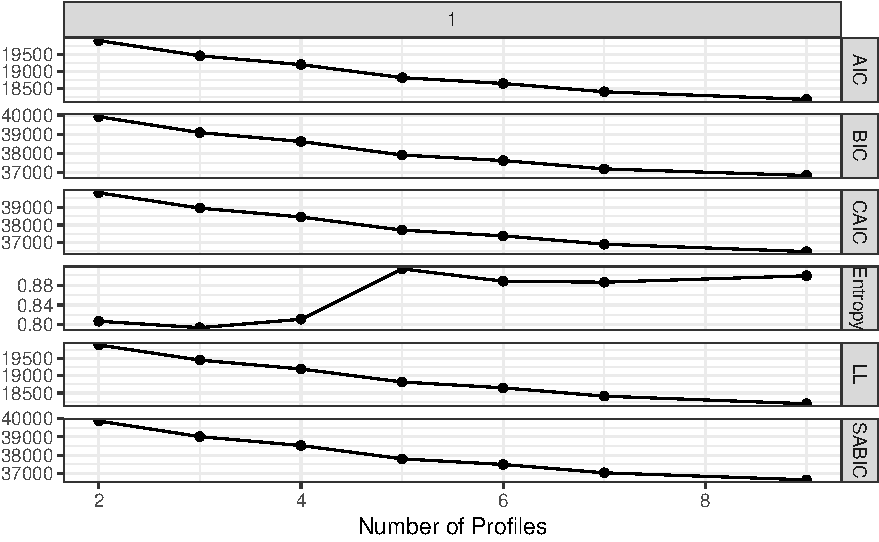
\includegraphics[width=0.5\linewidth]{rosenberg-dissertation_files/figure-latex/model1-1} 

}

\caption{Fit statistics for model 1 solutions}\label{fig:model1}
\end{figure}

\begin{figure}

{\centering 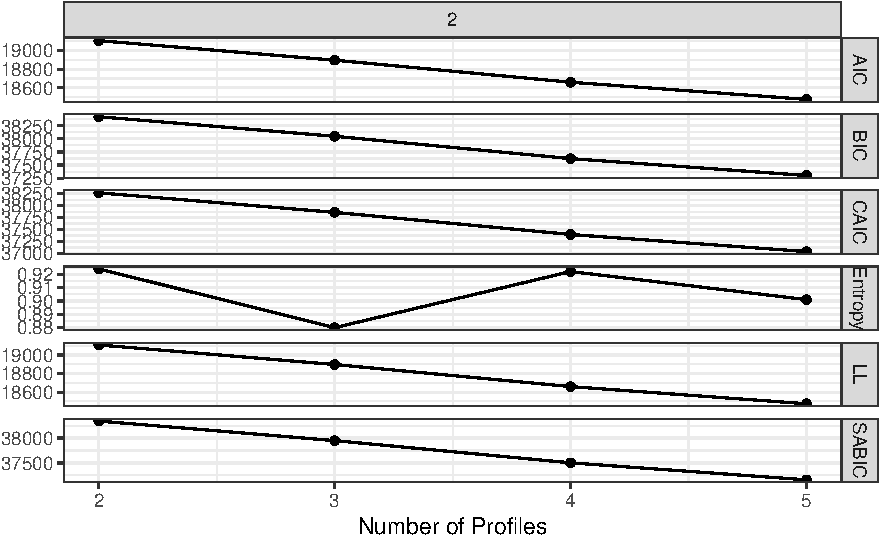
\includegraphics[width=0.4\linewidth]{rosenberg-dissertation_files/figure-latex/model2-1} 

}

\caption{Fit statistics for model 2 solutions}\label{fig:model2}
\end{figure}

For solutions associated with model 1, the decrease (indicating a
preferred model) in information criteria becomes smaller as the number
of profiles increases from 5 to 6 and 6 to 7. A solution associated with
8 profiles did not replicate the log-likelihood and the VLMR and LMR
suggest that the solution associated with 9 profiles did not fit better
than that with 8 profiles, suggesting that models with 7 or fewer
profiles be preferred. Considering these models, the entropy statistic
increases by a large amount between the solution associated with 4 and 5
profiles (and then decreases slightly between 5 and 6 and 6 and 7
profile solutions), suggesting (but not providing conclusive evidence)
that models 5, 6, or 7 may be preferred. The bootstrapped LRT suggests
that, until the log-likelihood is not replicated, every more complex
model be selected. Taking these pieces of evidence into conclusion, for
model 1, solutions associated with 4 through 7 may be considered in more
depth, with an emphasis on solutions associated with profiles with 5 and
6 profiles on the basis of the slowing of the decrease in the
information criteria associated with the solutions with greater profiles
than these, and the increase in the entropy from 4 to 5 (and 6) profile
solutions.

For solutions associated with model 2, only those associated with 2-5
profile solutions were associated with log-likelihoods that were
replicated. For these four models, the log-likelihood decreased in a
mostly consistent way, such that changes in the decrease are not as
evident as those associated with model 1. The entropy statistic
decreases from 2 to 3 profile solutions, increases from 3 to 4 profile
solutions, and then decreases slightly from 4 to 5 profile solutions,
providing some information that models associated with 4 profiles be
preferred to the others. All of the LRTs suggest that the more complex
model be selected, not providing clear information about which solutions
are to be preferred. On the basis of these pieces of evidence, models
with 3, 4, and 5 solutions may be considered in more depth. However,
there is a lack of consistent evidence favoring more or less complex
models.

The model 1, six and seven profile solutions are compelling because both
show profiles that are distinguished by dimensions of engagement and its
conditions (challenge and competence). Note that for this model, only
the means and variances are estimated (and so no covariances are
estimated), and the variances are constrained to be the same across the
profiles. While this is a very restrictive model, it, along with the
model 3 type (which did not lead to solutions for any of the numbers of
profiles specified) also is a standard model for LPA, in that it meets
the assumption of local independence (of the variables that make up the
profiles--unlike for models in which covariances are estimated) typical
common to LPA (see Muthen \& Muthen, 2016). While some of the solutions
associated with the model 2 type did reach solutions, these demonstrated
less appealing properties in terms of their fit statistics as well as
their interpretability and with respect to concerns of parsimony. Thus,
while no covariances are estimated for the model 1 type solutions, there
is no requirement that these be specified; their benefit, when models
associated with them are preferred, is that they can provide better fit:
they can be used to better explain or predict the data in a sample, but
their inclusion also means that over-fitting the model to the data can
become a greater concern.

For each solution, alternate solutions associated with higher
log-likelihoods were explored. One advantage of the six profile solution
is that most of its profiles can also be identified in solutions with
fewer profiles. For the six profile solutions, this alternate solution
was very different, whereas for the seven profile solutions, this
alternate solution was highly similar. The model solutions exhibit a
less clear pattern in terms of which profiles appear when. All else
being equal, on the basis of parsimony, the model 1, six profile
solution is preferred and was selected for use in subsequent analyses.

\subsection{Appendix F: Alternate model selected (model type 1, seven
profile
solution)}\label{appendix-f-alternate-model-selected-model-type-1-seven-profile-solution}

This solution is characterized by:

\begin{itemize}
\tightlist
\item
  A \emph{full} profile, profile 7
\item
  A \emph{universally low} profile, profile 1
\item
  A \emph{competent but not engaged or challenged} profile, profile 2,
  characterized by high competence and moderate (low) or low levels of
  engagement and challenge
\item
  A \emph{moderately low} profile, profile 3, characterized by
  moderately low levels of all of the variables
\item
  A \emph{challenged} profile, profile 4, characterized by high
  challenge, moderate (high) levels of engagement, and moderate (low)
  levels of competence
\item
  A \emph{highly challenged} profile, profile 5, characterized by
  patterns similar to those of the challenged profile, but with higher
  challenge and with low levels of both engagement and challenge
\item
  A \emph{challenged but not engaged or competent} profile, profile 6,
  characterized by low levels of challenge, and high levels of
  engagement and competence
\end{itemize}

\begin{center}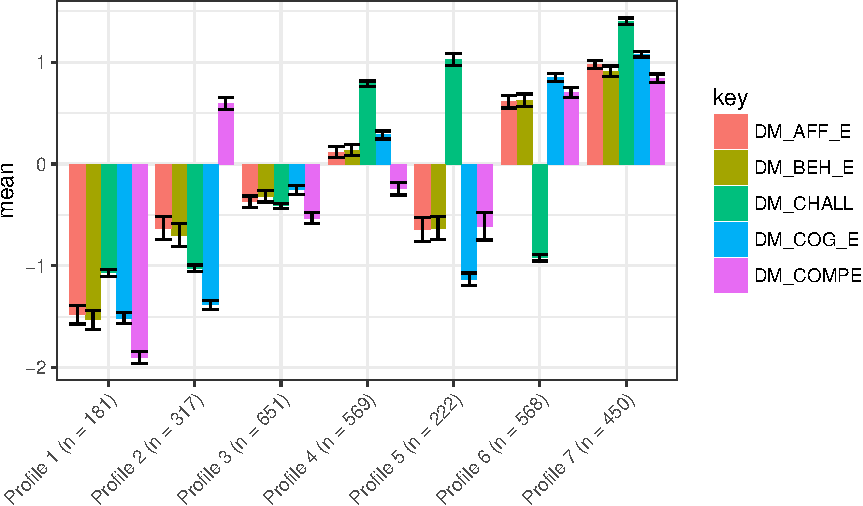
\includegraphics[width=0.9\linewidth]{rosenberg-dissertation_files/figure-latex/m1_7p-1} \end{center}

\begin{center}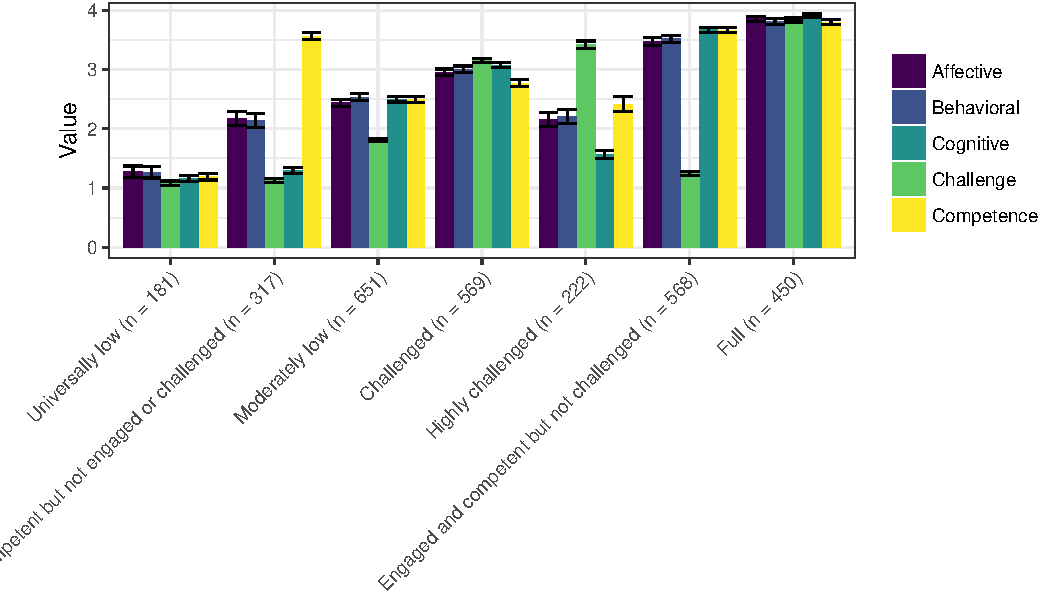
\includegraphics[width=0.9\linewidth]{rosenberg-dissertation_files/figure-latex/m1_7p-2} \end{center}

The number of observations associated with each of the profiles is not
very balanced, with few (\emph{n} = 181) observations associated with
the universally low profile and few (\emph{n} = 222) observations
associated with the highly challenged profile. The number of
observations associated with the other profiles ranged from 317 to 651.
Distinct from other solutions, none of the other five profiles were
found in the other model 1 solutions. Two pairs of the
profiles--challenged and highly challenged and universally low and
moderately low--exhibited similar patterns among the variables that were
distinguished by different mean levels. The log-likelihood was
replicated twice, with the next lowest log-likelihood being replicate
four times, possibly warranting further investigation. Taken together,
this solution raises questions about whether it may be too complex,
possibly suggesting preference for model 1 five and six profile
solutions.

\bibliography{book.bib,packages.bib}


\end{document}
